\section{Auswahl der Technologie - Client [DH] [BG]}
\setauthor{Benjamin Golic}

Da die Kennzeichenverwaltung und der Web-Shop plattformunabhängig eingesetzt werden sollen, ist die Entscheidung auf eine Web-Applikation gefallen.

Eine Web-Applikation ist eine Anwendung, die über das Internet abrufbar ist. Diese wird mittels Client-Server-Architektur umgesetzt. Bei dieser Architektur befinden sich die Daten und die Logikschicht auf einem Server und die Darstellung davon erfolgt im Webbrowser des Benutzenden.

Da Web-Applikationen lediglich einen Web-Browser erfordern, sind sie plattformübergreifend nutzbar und erfordern kein spezielles Betriebssystem.
Im Vergleich dazu, werden bei klassischen Softwarelösungen oftmals Betriebssysteme oder spezielle Programme vorausgesetzt, um auf die vollständige Funktionalität zurückgreifen zu können.

\subsubsection{Komponente: Webserver}
\setauthor{Benjamin Golic}
Web-Applikationen werden auf Webservern ausgeführt. Im einfachsten Fall wird nur ein Server genutzt, allerdings handelt es sich in der Praxis meist um mehrere Systeme. 

Grundsätzlich wird zwischen zwei Architekturen unterschieden, zum einen „Standalone“ und zum anderen „Integriert“. Bei der „Standalone“ – Architektur ist die Webanwendung ein Skript, das bei jeder Anfrage neu ausgeführt wird. Bei der „Integriert“ – Architektur ist die Webanwendung ein Teil des Webservers.

Für die Datenspeicherung werden Dateien oder Datenbankserver verwendet. Außerdem können benutzerbezogene Daten in Form von Cookies auf dem Clientrechner gespeichert werden.

\subsubsection{Komponente: Client}
\setauthor{Benjamin Golic}

Der Web-Client ist der Web-Browser, der mit dem Webserver mittels des Request-Response-Verfahrens kommuniziert. Hierbei sendet der Web-Browser einen HTTP-Header mit einem Request an den Webserver, und der Webserver antwortet darauf mit einer HTTP-Response. Ein Request kann beispielsweise die Nachfrage nach einem Webseiteninhalt sein. 

\subsubsection{Vorteile einer Webapplikation:}
\setauthor{Benjamin Golic}

\begin{itemize}
  \item Plattformunabhängig
  \item Keine zusätzlichen Installationen notwendig
  \item Wartungsarbeiten finden an der Anwendung auf dem Webserver statt, dies bedeutet, dass die Nutzenden keine Updates installieren müssen, um die neuen Versionen der Web-App nutzen zu können
\end{itemize}

\subsubsection{Nachteile einer Webapplikation:}
\setauthor{Benjamin Golic}

\begin{itemize}
  \item -	Konstant funktionsfähige Internetverbindung notwendig
  \item -	Da alle Daten auf einem Cloud-System gespeichert werden, sind bei einem Hackerangriff alle Daten in Gefahr
\end{itemize}
\cite{WebApplikation} \cite{WebClientServer} \cite{dvsw}

\subsection{Unterschied Framework und Library [BG]}
\setauthor{Benjamin Golic}

Generell verfolgen Frameworks und Libraries das gleiche Ziel, nämlich den Funktionsumfang eines Programmes zu erweitern. Jedoch gibt es grundlegende Unterschiede zwischen den beiden.

\subsubsection{Library:}
\setauthor{Benjamin Golic}

Bei Libraries handelt es sich um Sammlungen von Klassen und Funktionen. Diese können die Entwickelnden in den eigenen Code einbinden. Der Zugriff auf die Funktionen der Library erfolgen über die Programmierschnittstelle (API, kurz für Application Programming Interface). Dieser ist allerdings auf „öffentliche“ Funktionen begrenzt. „Private“ Funktionen arbeiten nur im Hintergrund.

\subsubsection{Framework:}
\setauthor{Benjamin Golic}

Frameworks sind eine spezielle Art von Libraries, die allerdings keine Funktionen enthalten. Frameworks liefern den Bauplan und das Grundgerüst für ein Programm.

\cite{LibFramw}

\begin{quote}
  „Das Framework stellt eine wiederverwendbare, gemeinsame Struktur für Anwendungen zur Verfügung. Entwickler binden das Framework in ihre eigenen Anwendungen ein und erweitern es so, dass es ihre bestimmten Anforderungen erfüllt.“
\end{quote} \cite{framevsL2}

\begin{figure}[H]
  \centering
  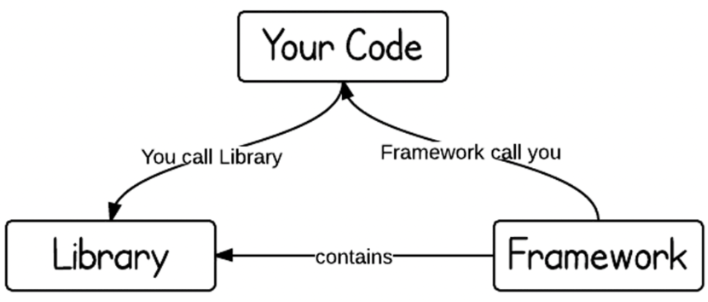
\includegraphics[width=0.8\textwidth]{pics/LibraryFramework.png}
  \caption{Unterschied zwischen der Funktionsweise eines Frameworks und einer Library}
  \cite{LibFramwImage}
\end{figure}

Um das Programmieren einer Web-Applikation zu erleichtern, wird auf JavaScript-Libraries und -Frameworks zurückgegriffen. Hier ist es möglich, zwischen vielen verschiedenen Möglichkeiten zu wählen. Die Wahl des richtigen Werkzeugs hängt von unzähligen Faktoren ab. Beispielsweise achten viele auf die Popularität oder auf die Etablierung. Für manche spielt auch die Unterstützung der Community eine wichtige Rolle bei der Entscheidung.

Die am häufigsten verwendeten JavaScript-Frameworks beziehungsweise -Libraries sind Angular, Vue.js und React.
\cite{framevsL2}

\begin{figure}[H]
  \centering
  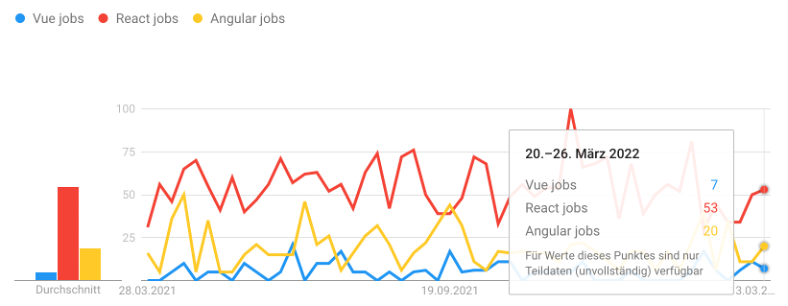
\includegraphics[width=0.8\textwidth]{pics/interesseFL.png}
  \caption{Interesse im zeitlichen Verlauf}
  \cite{InteresseGraph}
\end{figure}

Der größte Unterschied zwischen den drei populärsten JavaScript-Frameworks ist die Verwendung des DOMs (Document Object Model). React und Vue verwenden ein virtuelles DOM, wobei hingegen Angular auf das echte DOM setzt. Die Art des DOMs wirkt sich auf die Leistungsfähigkeit aus. Da bei dem virtuellem DOM die Nodes (Node-Schnittstellen sind die zentralen Objekte des DOMs) nur bei Bedarf neu geladen werden müssen, ist die Leistung deutlich besser im Vergleich zu echten DOMs.

Ein weiterer sehr großer Unterschied zwischen den Frameworks ist das Architekturmuster. Vue basiert auf dem Architekturmuster MVVM und Angular auf MVC, React hingegen basiert auf gar keinem Architekturmuster.
MVC steht für „Model View Controller“ und ist ein beliebtes Architekturmuster in der Programmentwicklung. Hierbei wird das Programm in drei Abschnitte aufgeteilt, in ein Model, eine Ansicht und eine Steuerung.

Das Model wird dazu verwendet, um die Logik der Anwendung zu implementieren. Es besteht aus mehreren Model-Klassen, wobei jede eine grundlegende Einheit innerhalb der verwendeten Datenstruktur verwendet. Des Weiteren stellen diese Klassen die grundlegenden Datenoperationen zur Verfügung.

Die View-Klassen sind für die grafische Benutzeroberfläche zuständig. Sie zeigen die von den Model-Klassen zur Verfügung gestellten Daten an, ohne eine direkte Verbindung aufzubauen.

Der Controller stellt ein Verbindungsstück zwischen den View- und Model-Klassen dar. Dieser ist für die Benutzeraktionen, die von der View weitergeleitet werden, zuständig.

\subsubsection{Vorteile von MVC:}
\setauthor{Benjamin Golic}

\begin{itemize}
  \item Ein Model kann in mehreren Views dargestellt werden
  \item Niedrige Kupplung
  \item Hohe Wiederverwendbarkeit
  \item Hohe Wertbarkeit
\end{itemize}

\subsubsection{Nachteile von MVC:}
\setauthor{Benjamin Golic}

\begin{itemize}
  \item Keine klare Definition
  \item Zu enge Verbindung zwischen View und Control
\end{itemize}
\cite{mvcBild} \cite{mvcVSmvvm}

\begin{figure}[H]
  \centering
  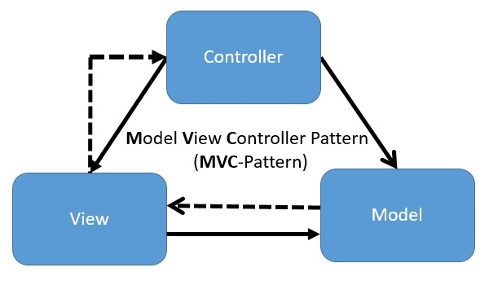
\includegraphics[width=0.8\textwidth]{pics/mvc.jpg}
  \caption{Aufbau des MVC-Patterns}
  \cite{mvcBild}
\end{figure}

MVVM steht für „Model-View-ViewModel“ und ist ebenfalls ein Software-Architekturmuster. Es besteht aus einem Model, einem ViewModel und einer View. 

Wie beim MVC enthalten die Model-Klassen die Daten. Das ViewModel fungiert als Verbindung zwischen Model und View. Es wandelt die Datenobjekte des Models so um, dass die View diese leichter darstellen kann. Ebenfalls wie beim MVC ist die View hier für die Benutzeroberfläche zuständig.

Der konzeptionelle Unterschied zwischen MVC und MVVM liegt darin, dass für MVC der Einstiegspunkt der Anwendung der Controller ist, während für MVVM der Einstiegspunkt die View ist.
\cite{mvcVSmvvm}

\begin{figure}[H]
  \centering
  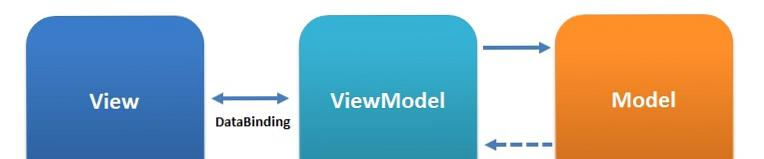
\includegraphics[width=0.8\textwidth]{pics/mvvm.jpeg}
  \caption{Aufbau des MVVM-Patterns}
  \cite{mvcVSmvvm}
\end{figure}

Schlussendlich sind Angular und React für das Frontend ausgewählt worden, wobei Angular für das Frontend der Systemverwaltung und React für den Web-Shop verwendet wurde. Diese Entscheidungen wurden von mehreren Faktoren beeinflusst. Die Hauptfaktoren hierbei waren die persönlichen Erfahrungen und Kompetenzen.

\subsubsection{Vorteile von MVVM:}
\setauthor{Benjamin Golic}

\begin{itemize}
  \item Logik kann unabhängig von der Darstellung bearbeitet werden
  \item Nützlich bei größeren Teamarbeiten
  \item Vereinfachte Testung der Komponenten
\end{itemize}

\subsubsection{Nachteile von MVVM:}
\setauthor{Benjamin Golic}

\begin{itemize}
  \item Data-Binding erschwert das Debugging
  \item	Das bidirektionales Data-Binding ist für Wiederverwendung von Code ungünstig
\end{itemize}

\cite{mvcBild} \cite{mvcVSmvvm}

\newpage

\subsection{Technologie zur Entwicklung des Frontends}
\subsection{Angular [DH]}
\setauthor{David Hauser}
Angular ist eines der großen Frameworks für Single-Page-Webanwendungen. Genauer genommen ist es ein sehr erfolgreiches, clientseitiges JavaScript-Web-Framework zur Erstellung von Single-Page-Webanwendungen. Mittlerweile hat sich Angular schon eher zu einer Plattform weiterentwickelt. Neben der reinen „API“ zur Anwendungsentwicklung beinhaltet Angular auch Entwicklungs-Werkzeuge, Generatoren und mitgelieferte Architektur-Konzepte. Es ist somit eine Ready-to-Rock Lösung, um Enterprise-Anwendungen zu entwickeln.

Angular wurde 2009 auf den Markt gebracht und konnte sich durch ihre Mission bei den vielen anderen Frameworks durchsetzen. Es ist ein wunderbares Ökosystem mit einer großartigen Community entstanden. Der Fokus auf Qualität und Enterprise ist dennoch zu spüren. Nach eigenen Angaben nutzt selbst Google das Framework in über 1600 Projekten.

\subsubsection{Das Ökosystem von Angular [DH]}
Die Plattform von Angular ist sehr groß. Die Basis dafür bietet das Core-Framework, in welchem fundamentale Konzepte implementiert sind, diese sind für moderne Webanwendungen essenziel. Die Angular CLI und die Verwaltung von Komponenten sind noch zwei weitere Core-Konzepte welche separat genutzt werden könnnen. Sie bilden die Kernfunktion und werden in fast allen Anwendungen benötigt. Einige weitere Module lassen sich noch einbinden:

\begin{itemize}
  \item Routing – Routing für Single Page Applications
  \item forms – Formulare und Validierung
  \item i18n – Mehrsprachige Anwendungen
  \item Animations – Animationen für Transitionen
  \item PWA – Offline Fähigkeiten
  \item HTTP – HTTP, Rest und GraphQL Kommunikation
  \item und noch unzählige mehr  
\end{itemize}
\cite{AngularBeschreibung}

\begin{figure}[H]
  \centering
  \includegraphics[width=0.8\textwidth]{pics/Ökosystem_Angular.png}
  \caption{Ökosystem von Angular}
  \cite{OekosystemAngularBild}
\end{figure}

\textit{Konsistenz}
Codekonsistenz ist ein wichtiges Ziel, welches bei der Programmierung mit Angular immer anzustreben ist. Das gesamte Framework basiert auf Komponenten und Diensten, welche in ihrem Aufbau immer gleich aussehen. Sie können sich wie ein Baustein vorgestellt werden. Alle Angular-Komponenten führen zu Beginn folgendes aus:

\begin{itemize}
  \item Import der erforderlichen ES-Module
  \item Definiton eines @Component-Dekorators
  \item Platzierung von Code in einer Komponentenklasse
\end{itemize}	

\begin{figure}[H]
  \centering
  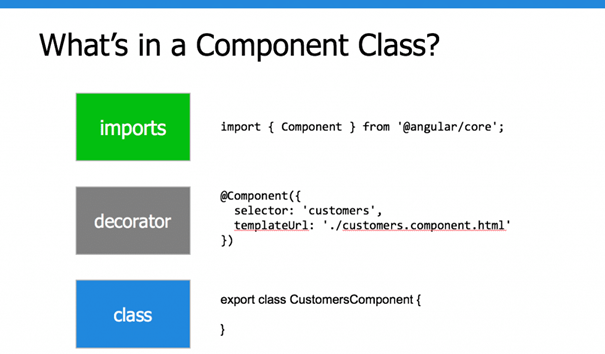
\includegraphics[width=0.8\textwidth]{pics/Komponenten_Klasse.png}
  \caption{Aufbau einer Komponente}
  \cite{AufbauKomponenteBild}
\end{figure}

Der Aufbau eines Bausteins ist immer gleich und unabhängig davon, welche Komponente geschrieben wird. Natürlich können einige Aspekte hinzugefügt werden, doch die Gesamtstruktur sieht immer gleich aus. Das sorgt von Anfang an für Konsistenz.

Services sind ein weiterer großer Bereich der Konsistenz in Angular. Diese sind ebenfalls wie Bausteine aufgebaut. In den Konstruktor einer Service-Klasse können alle Abhängigkeiten, die vom Service erfordert werden, eingefügt werden.

\begin{figure}[H]
  \centering
  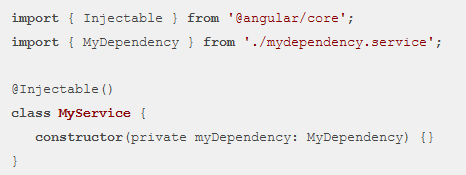
\includegraphics[width=0.8\textwidth]{pics/Code_Service.png}
  \caption{Beispielcode einer Service-Klasse}
\end{figure}

\subsubsection{Produktivität}
Die Produktivität rückt durch die Konsistenz in den Vordergrund, denn die Entwicklerin oder der Entwickler muss sich keine Gedanken darüber machen, ob er die Dinge auf die „richtige Weise“ macht. Komponenten und Services sehen gleich aus, wiederverwendbarer Anwendungscode wird in Serviceklassen abgelegt und ES-Module organisieren zugehörige Funktionen und ermöglichen, dass der Code self-contained und self-responsible ist. Daten werden mithilfe von Eingabeeigenschaften an Komponenten übergeben und lassen sich durch Ausgabeeigenschaften weitergeben.

\subsubsection{Wartbarkeit}
Angular hat den Vorteil, dass es von einer großen Community und deren Open-source-Beiträge, regelmäßig erweitert wird. Den größten Teil der Erweiterungen trägt allerdings Google bei. Es ist nie sicher, wie lange ein bestehendes System genutzt werden kann. Außerdem kommt es Angular zugute, dass sich Google über die Auswirkungen von etwaigen Änderungen bewusst ist. Da Google Angular selbst in Projekten verwendet, gibt es die Sicherheit, dass nichts schlagartig verändert oder die Wartung eingestellt wird. Neben der Unterstützung durch das Angular Team, ist auch die beschriebene Konsistenz ein Vorteil für die einfache Wartbarkeit.

\subsubsection{Modularität}
Angular organisiert den Code in sogenannten „Buckets“. Komponenten, Services, Pipes oder Anweisungen müssen in einem oder mehreren Buckets organisieren. Die Buckets werden in Angular als Module bezeichnet. Sie bieten die Möglichkeit, die Anwendungsfunktionalität zu organisieren und in Funktionen oder wiederverwendbare Abschnitte zu unterteilen. Module bieten außerdem noch andere Vorteile. 

\subsubsection{Frühzeitige Fehlererkennung}
TypeScript ist die Sprache zur Erstellung von Angular, was einige positive Aspekte mit sich bringt:

\begin{itemize}
  \item TypeScript ist keine eigenständige Sprache und somit eine Obermenge von JavaScript. Es kann vorhandener ES JavaScript Code verwendet werden und der Code funktioniert einwandfrei.
  \item Außerdem unterstützt TypeScript die wichtigsten ES-Funktionen.
  \item Typen werden von TypeScript unterstützt, und sind für eine frühzeitige Fehlererkennung enorm wichtig. Dadurch wird leichter erkannt ob etwas falsch übergeben oder verwendet wird.
  \item TypeScript Code kann direkt über den Browser debuggt werden.
  \item Bei TypeScript können ebenso Klassen und/oder funktionale Programmiertechniken verwendet werden.
\end{itemize}

Angular wurde ebenso mit dem Hintergedanken an Testbarkeit entwickelt. Die Angular-CLI macht den Prozess des Komponententests und des End-to-End Tests sehr einfach. Standardmäßig wird Karma und Jasmine dafür verwendet. Zudem können mit dem Befehl „ng test“ alle im Projekt vorhandenen Tests ausgeführt werden.

\cite{VorteileAngular}

\subsubsection{Nachteile von Angular}
\begin{itemize}
  \item Es gibt unterschiedliche Vorgehensweisen in Angular, um das gleiche Ziel zu erreichen. Deshalb ist es für den Programmierer oder die Programmiererin oft schwer, sich für den richtigen und effizientesten Weg zu entscheiden.
  \item Zudem sind die Lebenszyklusmethoden komplex, was sie nur schwer verständlich macht.
  \item Das Nutzen von Direktiven ist für die Manipulation des DOM sehr hilfreich, jedoch ist die Erstellung nicht gerade einfach.
  \item Das Erlernen von Angular ist aufgrund von nicht vollständiger und ausreichender Dokumentation etwas schwieriger.
\end{itemize}
\cite{NachteileAngular}

\subsection{Angular Materials}
Um das Design der Anwendung zu vereinfachen, wurde Angular Materials verwendet. Angular Materials sind moderne, schlichte Designkomponenten, mit denen unter relativ geringem Aufwand optisch ansprechende Anwendungen gestaltet werden können, welche sich auch auf allen Anzeigegeräten mit geringem Zusatzaufwand umsetzen lassen. \cite{AngularMaterials}

Objekte sollen in einem drei-dimensionalen Raum simuliert und eine natürliche, intuitive Darstellung und Interaktion ermöglichen. Bei der Entwicklung müssen dafür verschieden Prinzipien beachtet werden. 
\begin{itemize}
  \item Materialien besitzen eine einheitliche Höhe von 1dp, können aber in x- und y-Dimension verschieden sein.
  \item Der geworfene Schatten von Materialen ist je nach Höhe unterschiedlich.
  \item Materialien sind für die Darstellung von Inhalten, welche dynamisch veränderbar sind, zuständig. Es kann nur ein Teil von Materialien damit ausgefüllt werden, wobei der Platz durch dessen Dimensionen beschränkt ist.
  \item Materialien sind Festkörper und können nur an freien Positionen eingesetzt werden. Ihre Transformationen sind auf den freien Platz im Raum beschränkt.
  \item Sie dürfen ihre Form und Größe jederzeit ändern, wobei die zuvor genannten Einschränkungen zu beachten sind. Die Materialien sind trotzdem als fest anzusehen und dürfen nicht gefalten oder verbogen werden.
  \item Materialien können sich verbinden oder trennen.
\end{itemize}

Es werden von Angular Material bereits viele fertige Designideen angeboten. Diese müssen oftmals nur als css-Klasse oder Direktive angefügt werden.

\begin{itemize}
  \item Theming: Das Farbschemata kann mittels scss-Mixins einfach geändert werden. Um komplexere Änderungen vorzunehmen, können eigene Mixins erstellt werden.
  \item Elevation helpers: Die z-Positionen können durch css-Klassen oder Mixins einfach dargestellt werden. Es gibt auch ein Mixin für Animationen bei Höhenänderung.
  \item Typography: font-size, -height und -weight sind von css-Klassen vorgegeben, mithilfe von Mixins können auch diese verändert werden.
\end{itemize}

\begin{lstlisting}[caption=Hinzufügen von Angular Materials]
  npm install --save @angular/material @angular/cdk @angular/animations
\end{lstlisting}

Mit diesem Befehl wird Angular Material zum Projekt hinzugefügt.
Material: Dieses Standardpaket enthält die Materialkomponenten.
CDK (Component Dev Kit): Dieses Paket stellt dem Entwickler, komponentenunabhängige Werkzeuge zur Verfügung.
Animations:  Dieses Paket wird für erweiterte Animation benötigt.

Theme
Das Design von Angular Materials muss durch ein Theme definiert werden. Es kann eines der vorgefertigen verwendet oder auch eine eigenes definiert werden. Zur Auswahl bei den vorgefertigten Themes stehen:

\begin{itemize}
  \item deeppurple-amber.css
  \item indigo-pink.css
  \item pink-bluegrey.css
  \item purple-green.css
\end{itemize}
\cite{AngularMaterials}

\newpage

\subsection{React [BG]}
\setauthor{Benjamin Golic}
React, auch bekannt unter React.js oder ReactJS, ist eine Open-Source JavaScript-Library, die zur Realisierung moderner Benutzeroberflächen dient. Die Bibliothek wurde das erste Mal im Jahr 2011 in einem Facebook-Newsfeed verwendet. Im Jahr 2012 wurde sie dann bei Instagram eingesetzt und im darauffolgenden Jahr ist sie als Open-Source Projekt veröffentlicht worden. 

Die Grundeigenschaft von React ist, dass es komponentenbasiert ist. Das bedeutet, dass die Anwendung in logisch trennbare Einheiten unterteilt wird, die dann unabhängig voneinander behandelt werden können. Aus diesem Grund eignet sich React besonders gut für Single-Page-Applications.
\cite{WasIstReact}

\begin{lstlisting}[language=JavaScript, caption=Möglicher Aufbau einer Komponente in einer JavaScript-Funktion, label=lst:impl:aufbauJSFunction]
  function Welcome(props) {
    return <h1>Hello, {props.name}</h1>;
  }
\end{lstlisting} \cite{WasIstReact}

\begin{lstlisting}[language=JavaScript, caption=Möglicher Aufbau einer Komponente in einer JavaScript-Klasse, label=lst:impl:aufbauJSClass]
  class Welcome extends React.Component {
    render() {
      return <h1>Hello, {this.props.name}</h1>;
    }
  }
\end{lstlisting} \cite{WasIstReact}

\subsubsection{Single-Page-Applications:}
\setauthor{Benjamin Golic}

Single-Page-Applications bestehen im Gegensatz zu Multi-Page-Applications aus einem HTML-Dokument und können neue beziehungsweise veränderte Daten dynamisch laden. Da dies zu einer client-seitigen Verarbeitung der Anwendung führt, wird die Server-Client Kommunikation verringert.

Das dynamische Laden der Daten bedeutet, dass die Seite nicht aktualisiert beziehungsweise verlassen werden muss, da sich lediglich der Inhalt der aktuellen Ansicht clientseitig verändert.

Da nur eine Abfrage an den Server erfolgt, werden gleich alle Daten übermittelt. Aus diesem Grund ist es möglich, dass Nutzende sich durch die Website navigieren.

\cite{vergleichSPAundMPA} \cite{T3NReact}

\begin{figure}[H]
  \centering
  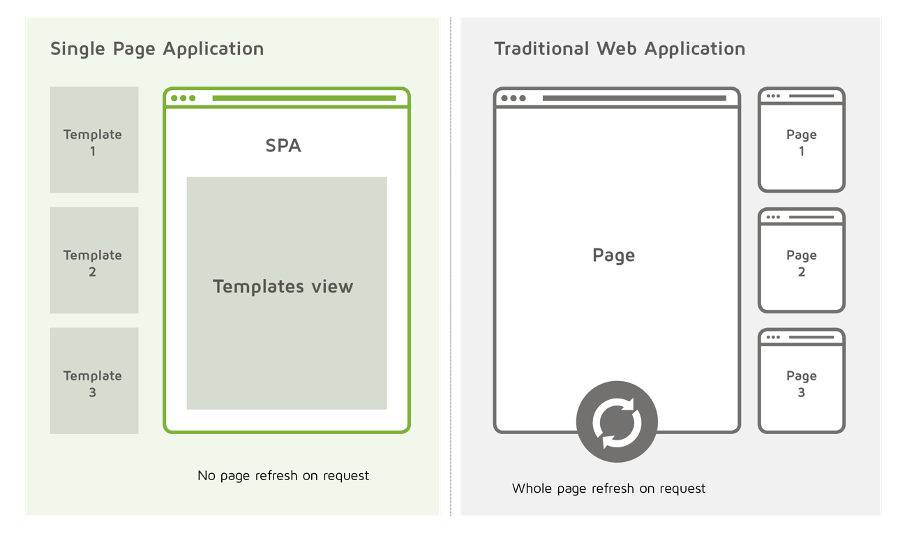
\includegraphics[width=0.8\textwidth]{pics/vergleichSPA-MPA.png}
  \caption{Aufbau einer Komponente}
  \cite{vergleichSPAundMPA}
\end{figure}

Der HTML-Source-Code einer Komponente wird in JavaScript-Klassen und -Funktionen geschrieben. Der ganze Source-Code wird hierbei mit der Syntaxerweiterung JSX geschrieben, wobei diese Erweiterung hauptsächlich für React entwickelt wurde.

Die Komponenten bestehen intern aus Properties und einem State. Außerdem werden sie in einer Baumstruktur angeordnet.
\cite{WasIstReact}

\begin{figure}[H]
  \centering
  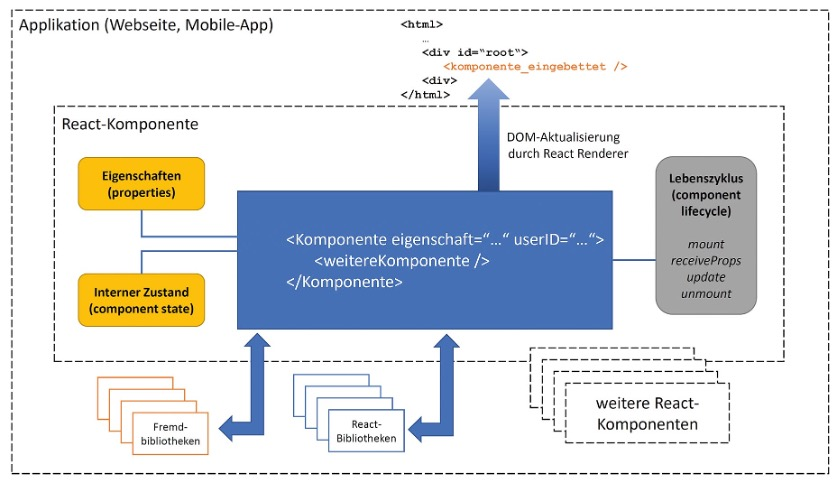
\includegraphics[width=0.8\textwidth]{pics/aufbauReactComponent.jpg}
  \caption{Aufbau einer Komponente}
  \cite{WasIstReact}
\end{figure}

\newpage

\subsubsection{JSX:}
\setauthor{Benjamin Golic}

JSX steht für JavaScript Syntax Extension beziehungsweise für JavaScript XML. Es ist eine Erweiterung der gewöhnlichen JavaScript-Grammatik für React. Bei der normalen JavaScript Grammatik wird JavaScript in Form von kleineren Scripten innerhalb einer HTML-Datei verwendet. Im Vergleich dazu ist das Ganze bei JSX genau umgekehrt, denn hier wird der HTML Code innerhalb der JavaScript-Klassen beziehungsweise Funktionen verwendet.

Damit der Browser die JSX-Dateien interpretieren kann, ist ein Präprozessor notwendig. Dieser wandelt den JSX-Code in gewöhnliches JavaScript um.
Bei der Umwandlung wird aus jedem HTML-Tag in der JSX-Datei ein Element mittels React.create erzeugt.

\cite{JSX}

\begin{lstlisting}[language=JavaScript, caption=JSX-Code, label=lst:impl:jsx]
  <MyButton color="blue" shadowSize={2}>
    Click Me
  </MyButton>
\end{lstlisting}\cite{JSX}

\begin{lstlisting}[language=JavaScript, caption=JSX-Code in gewöhnliches JavaScript kompiliert, label=lst:impl:jsxInJS]
  React.createElement(
    MyButton,
    {color: "blue", shadowSize: 2},
    "Click Me"
  )
\end{lstlisting}\cite{JSX}

Ein erwähnenswertes Merkmal von JSX ist, dass die Möglichkeit besteht, bestehende React-Komponenten über die Punkt-Notation innerhalb des JSX-Source-Codes aufzurufen.
\cite{JSX}

\subsubsection{Props:}
\setauthor{Benjamin Golic}
Props sind Eigenschaften, die an Komponenten übergeben werden. Diese Eigenschaften erweitern die Funktionalität. Sie können innerhalb der Komponente wie Variablen in Verwendung genommen werden.
\cite{PropsAndComponents} 

\begin{lstlisting}[language=JavaScript, caption=Komponente 'Welcome' die Props 'props' erwartet, label=lst:impl:componentWelcome]
  function Welcome(props) {
    return <h1>Hallo {props.name}</h1>;
  }
\end{lstlisting}\cite{PropsAndComponents}

\begin{lstlisting}[language=JavaScript, caption=Aufruf der Komponente 'Welcome' mit Übergabe des props 'name', label=lst:impl:UebergabeName]
  <Welcome name="Sara" />
\end{lstlisting}\cite{PropsAndComponents}

\begin{lstlisting}[language=JavaScript, caption=Ausgabe der Komponente 'Welcome', label=lst:impl:ausgabeComponentWelcome]
  Hallo, Sara
\end{lstlisting}

Bei der Verwendung von Props muss darauf geachtet werden, dass diese Read-Only sind.
\cite{PropsAndComponents2}

\subsubsection{State:]}
\setauthor{Benjamin Golic}
Eine weitere Besonderheit von React ist die Verwendung von States. Ein State ist die Beschreibung des Istzustands der Applikation. Beim Aufrufen der Website befindet sich diese in einem Initial State. Alle veränderbaren Daten einer Komponente, die einen Einfluss auf den Zustand der View haben, werden in der State Variable hinterlegt.
Sobald sich der State innerhalb einer Komponente verändert, wird die Seite neu gerendert, somit werden die veränderten Daten direkt angezeigt.
\cite{T3NReact}

\begin{lstlisting}[language=JavaScript, caption=Beispiel Code eines Click Counters mit der Nutzung on States, label=lst:impl:CountButton]
  class CountButton extends React.Component {
    constructor(props) {
      super(props);
      this.state={
        count: 0,
        text: "Click Counter"
      };
    }

    handleClick() {
      this.setState({
        count: this.state.count + 1
      });
    }

    render() {
      return (
        <div>
          <h2>{this.state.count}</h2>
          <button onClick={this.handleClick.bind(this)}>
            {this.state.text}
          </button>
        </div>
      );
    }
  }
\end{lstlisting} \cite{CountButtonExampleCode}

\newpage

\subsubsection{Map:}
\setauthor{Benjamin Golic}
Eine Map ist ein Datentyp, der zusätzlich zum Wert auch einen eindeutigen zugehörigen Key abspeichert. Aufgrund der Einzigartigkeit jedes gespeicherten Schlüssels ist es nicht möglich, dass doppelte Paare in einer Map gespeichert werden. Die Schlüssel dienen zum Nachschlagen der zugehörigen Daten.

Die map()-Methode wird in React hauptsächlich dazu verwendet, um Arrays durchzulaufen beziehungsweise um sie an der grafischen Benutzeroberfläche anzuzeigen. Beim Durchlaufen der Daten wird ein neues Array erstellt, indem die Methode eine bereitgestellte Funktion für jedes Element im aufrufenden Array aufruft.
\cite{Map}

\begin{lstlisting}[language=JavaScript, caption=Beispiel Code für die Nutzung der map()-Methode, label=lst:impl:mapMethode]
  const Users = () => {
  const data = [
    { id: 1, name: "John Doe" },
    { id: 2, name: "Victor Wayne" },
    { id: 3, name: "Jane Doe" },
  ];

  return (
    <div className="users">
      {data.map((user) => (
        <div className="user">{user}</div>
      ))}
    </div>
  );
};
\end{lstlisting} \cite{Map}

\subsubsection{React ohne JSX:}
\setauthor{Benjamin Golic}
Es besteht die Möglichkeit, React ohne JSX zu benutzen. Dies ist für Entwickelnde, die keine Kompilierung in der eigenen Entwicklungsumgebung durchführen möchten, empfehlenswert.
Da sich jedes JSX Element mittels des Aufrufes von „React.createElement(component, props, ...children)“ aufrufen lässt, ist es möglich alles im einfachen JavaScript umzusetzen.
\cite{JSX}

\begin{lstlisting}[language=JavaScript, caption=Beispiel Code 'Hello World' mit JSX, label=lst:impl:helloWorldJSX]
  class Hello extends React.Component {
    render() {
      return <div>Hello {this.props.toWhat}</div>;
    }
  }

  ReactDOM.render(
    <Hello toWhat="World" />,
    document.getElementById('root')
  );
\end{lstlisting} \cite{ReactWithoutJSX}

\begin{lstlisting}[language=JavaScript, caption='Hello World' mit einfachem JavaScript, label=lst:impl:helloWorldJSX]
  class Hello extends React.Component {
    render() {
      return React.createElement('div', null, `Hello ${this.props.toWhat}`);
    }
  }
  
  ReactDOM.render(
    React.createElement(Hello, {toWhat: 'World'}, null),
    document.getElementById('root')
  );
\end{lstlisting} \cite{ReactWithoutJSX}

Des Weiteren besteht die Möglichkeit React mit TypeScript zu benutzen, falls dies dem Anwendenden lieber ist als JavaScript. Hierfür gibt es TSX, dies ist die TypeScript Variante von JSX.

\begin{lstlisting}[language=JavaScript, caption=Beispiel-Code eines Click Counters in TSX label=lst:impl:TSXcounter]
  import * as React from 'react';

  export default class Counter extends React.Component {
    state = {
      count: 0
    };

    increment = () => {
      this.setState({
        count: (this.state.count + 1)
      });
    };

    decrement = () => {
      this.setState({
        count: (this.state.count - 1)
      });
    };

    render () {
      return (
        <div>
          <h1>{this.state.count}</h1>
          <button onClick={this.increment}>Increment</button>
          <button onClick={this.decrement}>Decrement</button>
        </div>
      );
    }
  }
\end{lstlisting} \cite{ReactWithoutJSX2}

\subsubsection{Arbeiten im Team mit React:}
\setauthor{Benjamin Golic}
Da alle Komponenten in einer eigenen Datei gespeichert werden, kann jedes Teammitglied beziehungsweise jedes kleinere Team in einem großen Projekt-Team für eine oder mehrere Komponenten verantwortlich sein. Dies verringert die Gefahr von Merge-Konflikten in Git und sorgt dafür, dass andere Teammitglieder den Code von anderen überschreiben.
\cite{PropsAndComponents2}

\subsubsection{Single-Responsibility-Prinzip:}
\setauthor{Benjamin Golic}
Bei großen React-Projekten wird in den meisten Fällen das Single-Responsibility-Prinzip angewendet. Dies bedeutet, dass die einzelnen Komponenten immer einen einzigen Existenzzweck haben sollen und nur eine Sache gleichzeitig tun sollen. Das Ganze dient dazu, dass die Komponenten wiederverwendet werden, wie zum Beispiel eine Suchleiste.
\cite{SRP}

\begin{figure}[H]
  \centering
  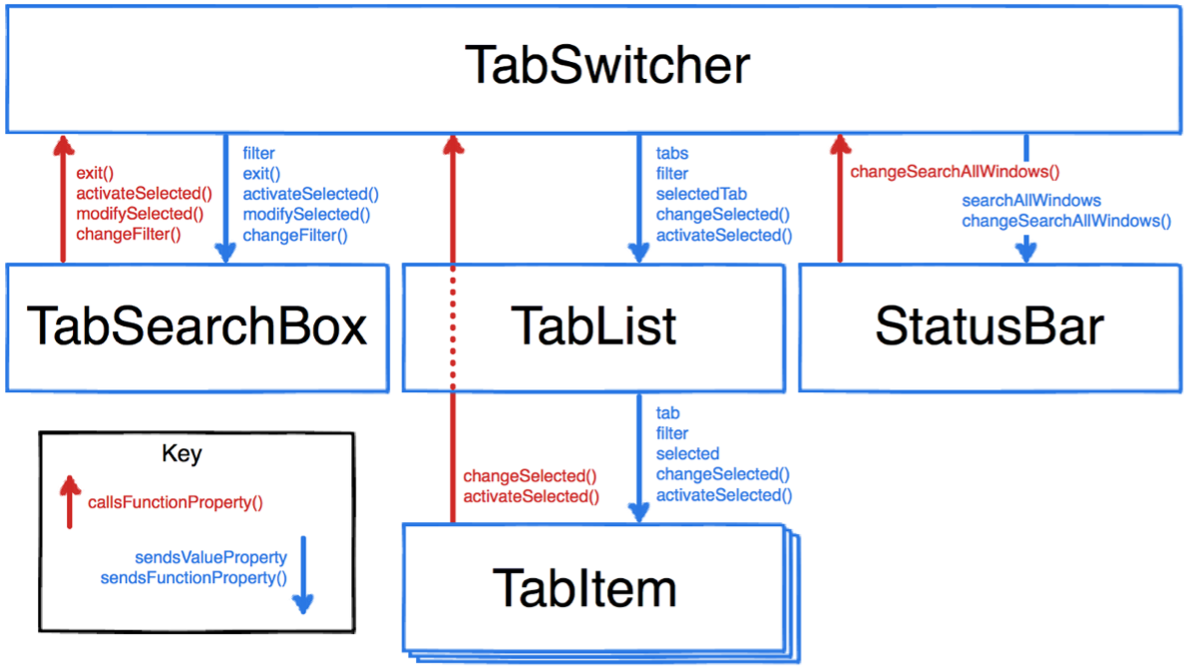
\includegraphics[width=0.8\textwidth]{pics/SRP.png}
  \caption{Beispiel für die Verwendung des Single-Responsibility-Prinzips}
  \cite{SRP}
\end{figure}

\newpage

\subsubsection{One Way Data Flow:}
\setauthor{Benjamin Golic}
React überträgt die Daten nur in eine Richtung zu den Komponenten, und zwar von „oben“ nach „unten“. Es werden nur Events, die von Nutzenden der Website ausgelöst werden, in gegenläufiger Richtung weitergegeben. Durch das Ganze sind Zusammenhänge und Wechselwirkungen einer Anwendung sehr überschaubar. Dies führt dazu, dass das Debugging vereinfacht wird.
\cite{owdf}

\begin{figure}[H]
  \centering
  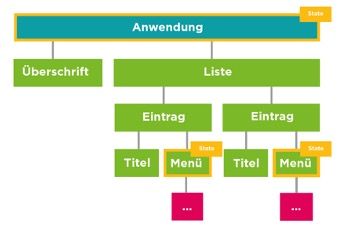
\includegraphics[width=0.8\textwidth]{pics/owdf.jpg}
  \caption{Darstellung des 'One Way Data Flow'}
  \cite{owdf}
\end{figure}

\subsubsection{Hooks:}
\setauthor{Benjamin Golic}
React Hooks bieten die Möglichkeit React-Funktionen, wie zum Beispiel State-Funktionen, in Function-Komponenten zu nutzen, dies war davor nur in Class- Komponenten möglich. Es gibt eine Reihe an unterschiedlichen Hooks.

Der wichtigste und am häufigsten verwendete Hook ist der State Hook. Er bietet die Möglichkeit, die State-Funktionalität in Function-Komponenten zu verwenden.

\cite{hooks}

\newpage

\begin{lstlisting}[language=JavaScript, caption=Code-Beispiel für Nutzung des State Hooks, label=lst:impl:stateHook]
  import React, { useState } from 'react';

  function Example() {
    const [count, setCount] = useState(0);

    return (
      <div>
        <p>Du hast mich {count} mal geklickt</p>
        <button onClick={() => setCount(count + 1)}>
          Klick mich
        </button>
      </div>
    );
  }
\end{lstlisting} \cite{hooks}

Die Funktion 'useState' liefert ein Array zurück, das in zwei Konstanten aufgeteilt wird. Die erste Konstante ist die Repräsentation des aktuellen States. Die zweite Konstante ist eine Funktion, die es ermöglicht, den aktuellen State zu verändern. Die Benennung dieser Konstanten spielt keine Rolle, da es sich um normale JavaScript-Konstanten handelt. Die Funktion 'useState' bekommt den Initial State als Argument übergeben.

Ein weiterer sehr wichtiger Hook ist der Effect Hook. Dieser Hook wird hauptsächlich für Änderungen verwendet, die bisher in Lifecycle-Methoden ausgeführt wurden. Dies bedeutet, dass bestimmte Änderungen durchgeführt werden, nachdem die Benutzeroberfläche gerendert wurde.
\cite{hooks}

\begin{lstlisting}[language=JavaScript, caption=Code-Beispiel für Nutzung des Effect Hooks, label=lst:impl:effectHook]
  import React, { useState, useEffect } from 'react';

  function Example() {
    const [count, setCount] = useState(0);
  
    // Similar to componentDidMount and componentDidUpdate:
    useEffect(() => {
      // Update the document title using the browser API
      document.title = `You clicked ${count} times`;
    });
  
    return (
      <div>
        <p>You clicked {count} times</p>
        <button onClick={() => setCount(count + 1)}>
          Click me
        </button>
      </div>
    );
  }
\end{lstlisting} \cite{hooks2}

Der Funktion 'useState' wird eine Funktion übergeben, die jedem neuen Rendering der Benutzeroberfläche ausgeführt wird.

Weitere Hooks:

\begin{figure}[H]
  \centering
  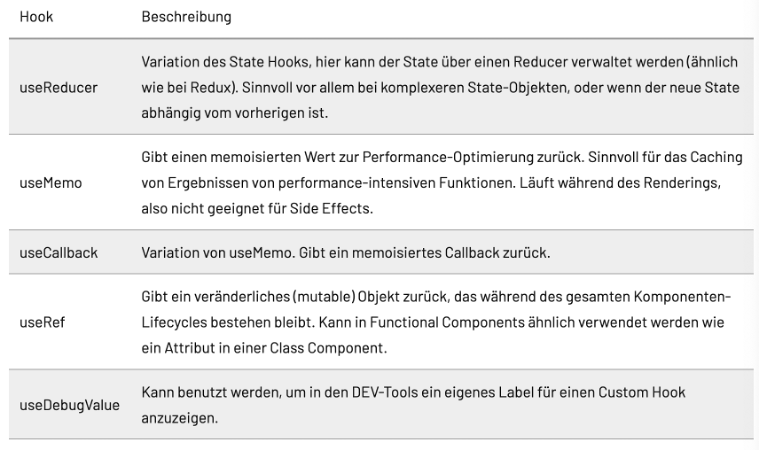
\includegraphics[width=0.8\textwidth]{pics/rHooks.png}
  \caption{Übersicht weiterer React-Hooks}
  \cite{hooks}
\end{figure}

\section{Auswahl der Technologie - Datenbank[SK]}
\setauthor{Simon Koll}
Die Datenbank spielt für das Projekt eine wichtige Rolle, daher wurden hier folgende Kriterien aufgestellt:

\begin{itemize}
  \item Das Projekt besteht aus Hard- und Software, die Daten sowohl abspeichern, als auch abfragen. Das kann je nach Anwendungsfall unterschiedlich sein.
  \item Vom Dashboard können beispielsweise Kennzeichen mit Gültigkeitsdauer, aber auch nur einfache NFC-Codes gesendet werden.
  \item In der Zukunft soll die Möglichkeit bestehen, weitere Zutrittsmöglichkeit hinzuzufügen. Daher muss sich die Datenbank der sich ändernden Datenstruktur anpassen können.
\end{itemize}

\subsection{Relationale Datenbanken}

Das Team befand sich vor der Entscheidung, ein relationales Datenbanksystem zu verwenden, oder ein nicht relationales Datenbanksystem.
Die größten Unterschiede hierbei sind, dass bei relationalen SQL-Datenbanken den gespeicherten Daten Tabellen vorgegeben sind, das sogenannte Schema. Das ist bei NoSQL-Datenbanken ebenfalls möglich, jedoch optional.
Relationale Datenbanken verfolgen das ACID-Prinzip. ACID steht für

\begin{itemize}
  \item \textit{Atomicity}
  \subitem Alle Änderungen der Datenbank werden als einzige Operation verarbeitet. Entweder werden alle Änderungen wie Inserts, Updates usw. durchgeführt, oder keine davon.
  \item \textit{Consistency}
  \subitem Zu Beginn und zum Ende jeder Transaktion sind die Daten konsistent.Beispielsweise bei einer Geldüberweisung, ist bei "Consistency" die Gesamtsumme der Geldmittel auf beiden Konten am Anfang und am Ende jeder Transaktion gleich.
  \item \textit{Isolation}
  \subitem Andere Transaktionen haben keine Einsicht in die Transaktion. Isolation bedeutet also, dass parallel laufende Transaktionen sich wie serialisierte verhalten.
  \item \textit{Durability}
  \subitem Die Daten bleiben nach Ende der Transaktion bestehen und werden auch bei einem kompletten Systemausfall nicht revidiert.
\end{itemize}
\cite{ACID}

\subsection{MongoDB}
Das Team entschied sich für eine der bekanntesten NoSQL-Datenbanken, \textbf{MongoDB}. Diese bietet einige Vorteile gegenüber den relationalen SQL-Datenbanken:

\begin{itemize}
  \item \textit{Skalierbarkeit: } MongoDB Datenbanken zeichnen sich durch ihre ausgezeichnete horizontale Skalierbarkeit aus. Horizontale Skalierbarkeit bedeutet, dass die Datenbank sich problemlos über mehrere Server verteilen kann, ohne die Funktionsfähigkeiten zu beeinträchtigen.
  \item \textit{Verfügbarkeit: } Die Datenbank muss immer zur Verfügung stehen, da  Abfrage ausgeführt wird.
  \item \textit{Flexibilität: } Da das Projekt weiterentwickelt werden kann, muss die Datenbank sich anpassen können.
\end{itemize}
\cite{VorteileMongoDB}
\section{Auswahl der Technologie - Kennzeichenerkennung[SK]}
\setauthor{Simon Koll}
Das Herz von APERTA ist die Kennzeichenerkennung. Dieses Alleinstellungsmerkmal separiert das Projekt von möglicher Konkurrenz. Dabei spielen Faktoren wie der Aufnahmewinkel der Kamera, die Distanz zum Kennzeichen, sowie die Lichtsituation eine entscheidende Rolle. Weiters muss aus den Einzelbildern der Kamera das Kennzeichen erkannt werden und danach die Buchstaben aus dem Bild extrahiert werden. Um dies zu vollbringen, werden 2 Libraries verwendet.
\subsection{OpenCV: } OpenCV steht für Open Source Computer Vision und ist eine frei Zugängliche Library, welche meist in Bereichen wie Machine Learning oder Machine Vision ihren Einsatz findet. Unternehmen können kostenlos auf die Bibliothek zugreifen, sie verändern und weiterentwickeln. Die Basis bilden die mehr als 2500 klassischen und neuen Algorithmen für das maschinelle Sehen. Diese haben unterschiedliche Spezialisierungen, wie unter anderem die Erkennung von Gesichtern, Objekten und Kamerabewegungen, die Generierung von 3D-Modellen, Ähnlichkeiten in Bildern zu finden, sowie Markierungen in Augmented Reality anzuzeigen. Zu den mehr als 18 Millionen Downloads und mehr als 47.000 Benutzern oder Benutzerinnen zählen meist Unternehmen, Forschungsgruppen oder Regierungsstellen. Bekannte Namen hier sind Google, Microsoft, Intel oder Sony.\cite{AboutOpenCV}
OpenCV hat eine modulare Struktur, was bedeutet, dass das Paket mehrere gemeinsam genutzte oder statische Bibliotheken enthält. Die folgenden Module sind verfügbar:
\begin{itemize}
    \item Kernfunktionalität (core) - ein kompaktes Modul, das grundlegende Datenstrukturen definiert, darunter das dichte mehrdimensionale Array Mat und grundlegende Funktionen, die von allen anderen Modulen verwendet werden.
    \item Bildverarbeitung (imgproc) - ein Bildverarbeitungsmodul, das lineare und nichtlineare Bildfilterung, geometrische Bildtransformationen (Größenänderung, affines und perspektivisches Warping, generisches tabellenbasiertes Remapping), Farbraumkonvertierung, Histogramme usw. umfasst.
    \item Videoanalyse (Video) - ein Videoanalysemodul, das Algorithmen zur Bewegungsschätzung, Hintergrundsubtraktion und Objektverfolgung umfasst.
    \item Kamerakalibrierung und 3D-Rekonstruktion (calib3d) - grundlegende Geometriealgorithmen für mehrere Ansichten, Einzel- und Stereokamerakalibrierung, Objektposenschätzung, Stereokorrespondenzalgorithmen und Elemente der 3D-Rekonstruktion.
    \item 2D Features Framework (features2d) - Erkennung auffälliger Merkmale, Deskriptoren und Deskriptor-Matcher.
    \item Objekterkennung (objdetect) - Erkennung von Objekten und Instanzen der vordefinierten Klassen (z. B. Gesichter, Augen, Tassen, Menschen, Autos usw.).
    \item High-Level-GUI (highgui) - eine leicht zu bedienende Schnittstelle zu einfachen UI-Funktionen.
    \item Video I/O (videoio) - eine einfach zu bedienende Schnittstelle für Videoaufnahmen und Videocodecs.
    \item Einige andere Hilfsmodule, wie z.B. FLANN- und Google-Test-Wrapper, Python-Bindings, und andere.
\end{itemize}
 \subsection{Tesseract: } Tesseract ist eine Texterkennungs-Engine welche von Google entwickelt wird. 

 Optische Zeichenerkennung oder Optical Character Reading (OCR) ist die elektronische oder mechanische Umwandlung von Bildern mit getipptem, handgeschriebenem oder gedrucktem Text in maschinell kodierten Text, sei es aus einem gescannten Dokument, einem Foto eines Dokuments, einem Szenenfoto (z. B. der Text auf Schildern und Werbetafeln in einem Landschaftsfoto) oder aus einem Untertiteltext, der einem Bild überlagert ist (z. B. aus einer Fernsehsendung).
 \cite{ocrWiki}

Um besser zu verstehen, wie OCR funktioniert, hilft dieses Prozessdiagramm in der folgenden Abbildung. Aus Sicht von Endbenutzern oder Endbenutzerinnen ist der OCR-Prozess einfach: Er verarbeitet das Bild und erhält den bearbeitbaren Text.
\begin{figure}[H]
  \centering
  
\includegraphics[width=10cm]{pics/OCR-Prozessdiagramm.png}
  \caption{Prozessdiagramm der Optische Zeichenerkennung}
  \cite{introToTesseract}
\end{figure}
 Tesseract bietet die Möglichkeit, Text aus Bildern zu extrahieren. Dies kann in vielen verschiedenen Programmiersprachen erfolgen, oder über eine graphische Nutzeroberfläche eines Drittanbieters.\cite{AboutTesseract} Unterstützt wird Tesseract durch einen Python-Wrapper mit dem Namen \textbf{pytesseract}, welcher Bilder wie .jpeg, .png, .gif und viele mehr laden kann, sowie den gelesenen Text ausgeben kann, anstatt ihn in einer Datei abspeichern zu müssen.\cite{AboutPyTesseract}
 
\section{Auswahl der Technologie - Backend[SK]}
\setauthor{Simon Koll}
\subsection{Anforderungen an das Backend}
Für das Backend kamen mehrere Technologien in Frage, wie unter anderem Java, JavaScript, Python, PHP, C$\sharp$, und viele mehr.
Um das Backend zu realisieren, muss die Technologie einige bestimmte Eigenschaften besitzen.\cite{CompareBackendLanguage}
\begin{itemize}
    \item \textit{Java:}
    \subitem Die Vorteile von Java liegen in der Fehlerbehandlung, sowie in Bereichen wie Multithreading und Performanz. Die strikte Fehlerbehandlung führt dabei aber zum Verlust von Flexibilität und Kompaktheit des Codes.
    \item \textit{JavaScript:}
    \subitem Die Syntax von JavaScript ähnelt der von Java. Entwickelt als Scripting-Sprache für HTML, ist JavaScript einfach zu lernen und zu benutzen. Bei der Entwicklung von Websites kann JavaScript direkt in den Quellcode der HTML-Seite eingearbeitet werden. Aber auch im Backend-Bereich kann mit NodeJS in JavaScript entwickelt werden.
    \item \textit{Python:}
    \subitem Python ist eine der mit Abstand am leichtesten zu lesenden Programmiersprachen. Die flache Hierarchie ermöglicht ein einfaches Verständnis von Programmen und Codestücken. Weiters macht Python Entwickler oder Entwicklerinnen auf Fehler aufmerksam, wenn dieser nicht ausdrücklich ignoriert werden soll.
    Jedoch ist Python manchmal langsamer in der Ausführung, als die konkurrierenden Sprachen. Zusätzlich ist durch die Verwendung von Leerzeichen zur Einrückung ein häufiger Fehlergrund hinzugekommen.
    \item \textit{PHP:}
    \subitem Die PHP Syntax erinnert an eine Mischung aus C, Java und Perl. Das Ziel von PHP ist es, Entwickler oder Entwicklerinnen schnell und einfach dynamisch generierte Webpages bauen zu lassen. Die vermischte Syntax ist jedoch etwas chaotisch, darum ist es leicht, sich in falschen Angewohnheiten zu verirren und Sicherheitslücken offen zu lassen.
  \end{itemize}
  Aufgrund vorhandener Vorkenntnisse standen für das Team 3 der oben genannten Technologien zur Auswahl:

  \begin{itemize}
    \item Java,
    \item JavaScript und
    \item Python
  \end{itemize}

  \subsection{Verwendung von NodeJS}
  Von diesen konnte sich JavaScript durchsetzen. Die Gründe dafür waren:\cite{WhyNodeJs}
  \begin{itemize}
    \item NPM:
    Der NPM oder \textit{Node Package Manager}, ist ein Paketmanager für JavaScript, welcher bei NodeJS standardmäßig mitgeliefert wird. Bei NPM werden wiederverwendbare Programmteile veröffentlicht. Diese können mittels des NPM eingenen Command Line Interfaces installiert werden. Weiters bietet der NPM eine integrierte Versionsverwaltung der Pakete, sowie eine Verwaltung der Abhängigkeiten.
    In diesem Projekt wurden beispielsweise die Module \textit{express} und \textit{mongodb} verwendet. \\
    \textit{express} ist ein Framework, welches vor allem in NodeJS Projekten verwendet wird. Die Vorteile von Express sind unter anderem die dem Team bereits bekannte Programmiersprache JavaScript, die Unterstützung der Google V8 engine für bessere Performance, die Robustheit bei einer Vielzahl an HTTP-Anfragen, sowie die einfache Einbindung weiterer Module und Drittanbieterapplikationen. \cite{WhyExpress}\\
    \textit{mongodb} stellt Entwicklern pder Entwicklerinnen eine API zur Verfügung, welche die Nutzung einer MongoDB-Datenbank stark vereinfacht.
    \item Verwendung einer NoSQL Datenbank:
    Aufgrund des Formates, mit dem die Daten aus dem Frontend kommen, bat sich eine nicht relationale Datenbank für das Team an. Die dokumentenorientierte Datenbank MongoDB ist bekannt für ihre hohe Verfügbarkeit, sowie für die gute Skalierbarkeit.
    \cite{WhyMongoDB}
    \item Behandlung von JSON:
    NodeJS zeichnet sich durch seine einfache Verwendung von JSON-Daten aus. Diese können ohne Parsing oder andere Konvertierungen verarbeitet und darauf zugegriffen werden. Dank NodeJS können JSON Objekte mittels REST-API Anfragen direkt für den Client bereitgestellt werden.
    Dank NodeJS kann eine einfache Verbindung zwischen Frontend-Clients und dem Backend-Server geschaffen werden.
  \end{itemize}

\section{Auswahl der Technologie - Hardware[SK]}
\setauthor{Simon Koll}
\subsection{Anforderungen an die Hardware}
Das Projekt sollte so vielseitig wie möglich, jedoch auch so kompakt wie möglich sein. Dazu musste auf kleine Komponenten gesetzt werden. Diese sollen dennoch leistungsfähig genug sein, um jede der drei Zugangsmöglichkeiten parallel zu verwalten.
\subsubsection{Raspberry Pi}
Die Wahl des Herzstückes fiel auf einen Raspberry Pi.
Der Raspberry Pi ist ein vollwertiger Computer, welcher etwas größer als eine Kreditkarte ist. Er besitzt alle bekannten Anschlüsse eines normalgroßen PCs, wie HDMI-Ausgänge für Monitore, USB-Ports für Peripherie wie Maus, Tastatur oder Webcams, sowie einen LAN-Port für eine kabelgebundene Netzwerkverbindung.
Als Betriebssystem des Raspberry Pi wurde das vom Hersteller empfohlene Raspbian OS verwendet. Dieses bietet eine grafische Benutzeroberfläche, sowie die Möglichkeit den Raspberry auch ohne angeschlossenen Monitor betreiben zu können. \cite{WhatIsRaspberryPi}
\begin{figure}[H]
  \centering
  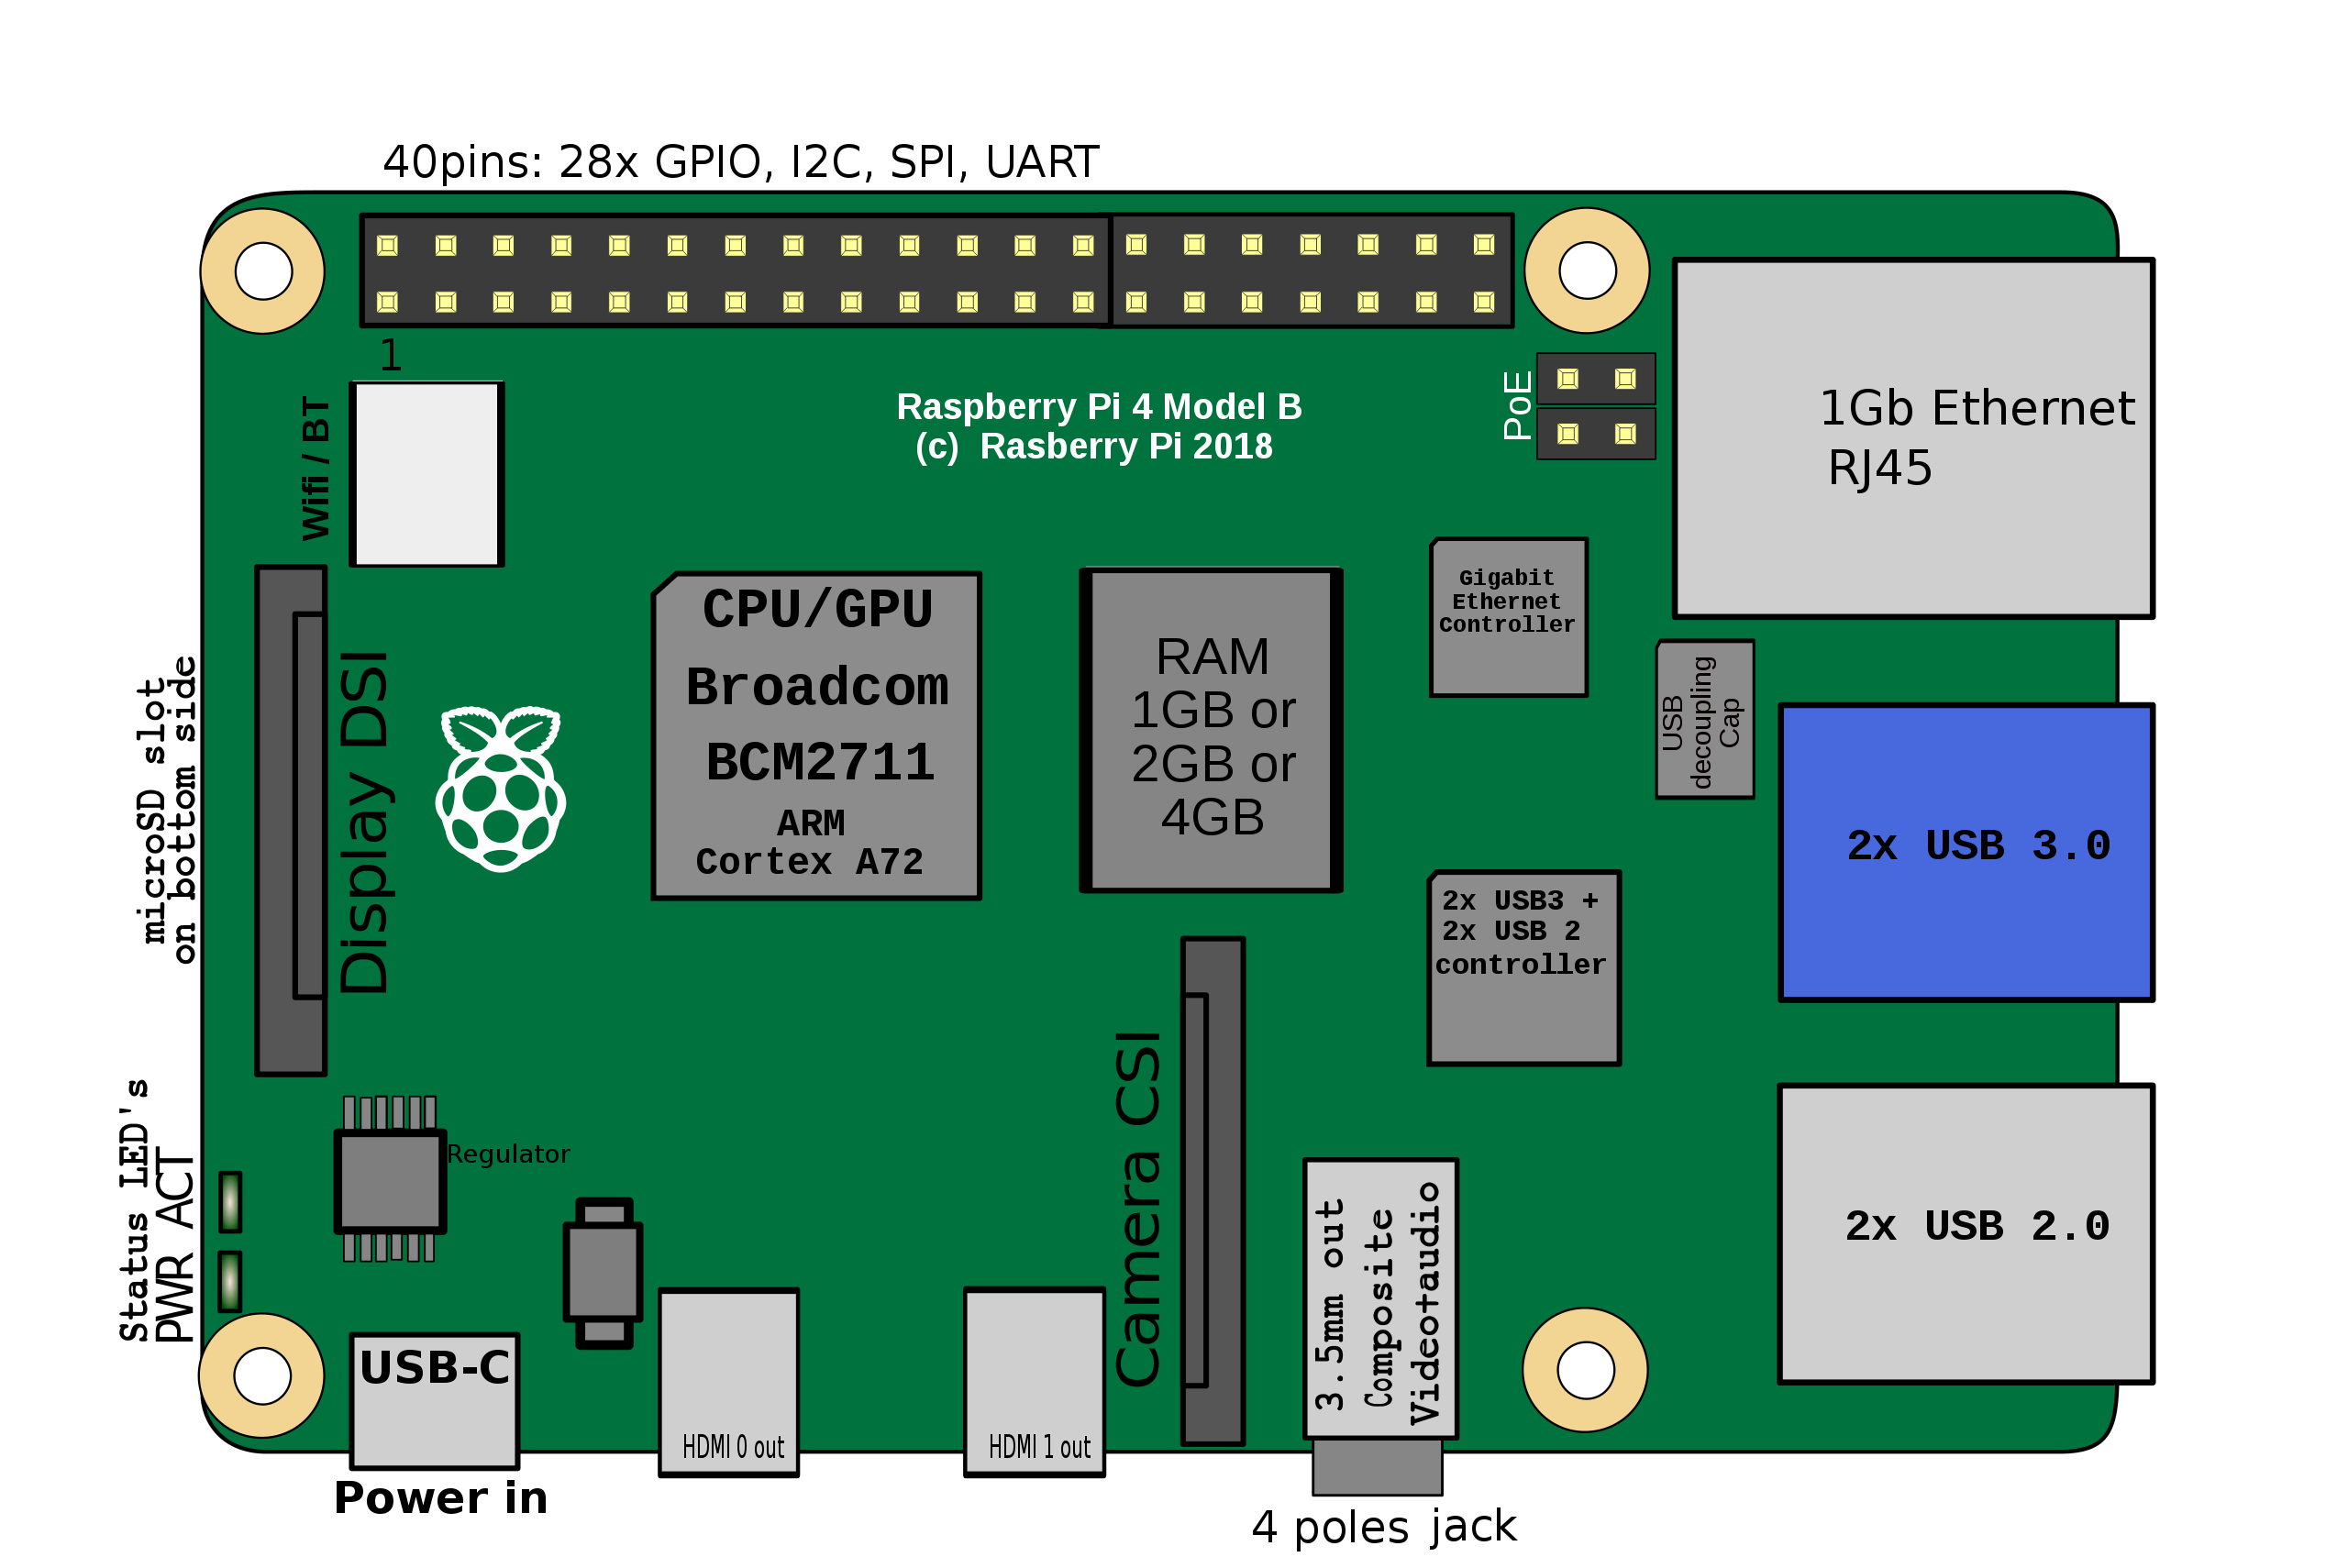
\includegraphics[width=10cm]{pics/2560px-RaspberryPi_4_Model_B.svg.png}
  \caption{Komponenten eines Raspberry Pi}
  \cite{RaspberryImage}
  \end{figure}


Auszeichnungsmerkmale des Raspberry Pi sind unter anderem die geringen Anschaffungskosten von ab EUR 35,00, sowie seine leistungsstarken Komponenten.\\
%\textbf{Bestandteile des Raspberry Pi} 
\begin{table}[H]
  \centering
  \caption{Übersicht der Komponenten des Raspberry Pi \cite{RaspySpecs}}
  \label{Komponenten des Raspberry Pi}
    \begin{adjustbox}{width=\textwidth}
      \begin{tabular}{lll}
      \hline
      \textbf{Komponente}                    & \textbf{Spezifikation}                                                    & \textbf{Besonderheiten}                    \\ \hline
      \multicolumn{1}{l|}{\textbf{Prozessor}} &
        \begin{tabular}[c]{@{}l@{}}Broadcom BCM2711\\ - Quad Core Prozessor @ 1.5GHz\end{tabular} &
        \begin{tabular}[c]{@{}l@{}}ARM Architektur\\ 64-Bit SoC\end{tabular} \\ \hline
      \multicolumn{1}{l|}{\textbf{RAM}}      & 1GB, 2GB, 4GB oder 8GB LPDDR4 SDRAM                                                          & Tatktung von 3200MHz                       \\ \hline
      \multicolumn{1}{l|}{\textbf{USB}}      & \begin{tabular}[c]{@{}l@{}}2 USB 3.0 Ports\\ 2 USB 2.0 Ports\end{tabular} &                                            \\ \hline
      \multicolumn{1}{l|}{\textbf{GPIO}}     & 40 Pin Header                                                             & Abwärtskompatibel mit Vorgängermodellen    \\ \hline
      \multicolumn{1}{l|}{\textbf{Display}}  & 2 micro-HDMI Ports                                                        & jeweils bis zu 4k60 möglich                \\ \hline
      \multicolumn{1}{l|}{\textbf{Speicher}} & Micro-SD Kartenslot                                                       & Speicherplatz für Betriebssystem und Daten \\ \hline
      \multicolumn{1}{l|}{\textbf{Strom}} &
        \begin{tabular}[c]{@{}l@{}}5V Eingang über USB-C Port\\ 5V Ausgang über GPIO-Header\end{tabular} &
        Anforderung an Stromquelle: mindestens 3A \\ \hline
      \end{tabular}
    \end{adjustbox}
  \end{table}
Der Raspberry Pi ist einer der am weitest verbreiteten Ein-Platinen-Computer der Welt. Trotz der im Verhältnis zu größeren Systemen schwachen Leistung wurde er im Jahr 2020 mehr als 7 Millionen mal verkauft worden. Daraus ergibt sich ein Marktanteil von allen PCs von 2.69\%.
Für ein ausgewogenes Verhältnis zwischen Kompaktheit und Leistung wurde auf einen Raspberry Pi 4 Model B in der Ausführung mit 4GB Arbeitsspeicher zurückgegriffen. Weiters waren die Anschaffungskosten von etwa 100\$ ein Grund für die Auswahl. \cite{RaspyMarketShare}

\textbf{Kernkomponenten des Raspberry Pi}\\
\textit{GPIO-Header}\\
Eine der Kernkomponenten, die den Raspberry Pi von anderen PC-Systemen unterscheidet, ist der "GPIO-Header". GPIO steht für General Purpose Input / Output, und kann wörtlich zu "Allzweckeingabe bzw. -ausgabe" übersetzt werden. Sie bezeichnen selbst programmierbare Ein- und Ausgänge, die auf dem Raspberry Pi als angelötete Pins zur Verfügung stehen.
Der Raspberry kann über diese Schnittstellen digitale Signale von außen annehmen, sowie auch Signale abgeben.
Der Raspberry Pi in der Ausführung Model 4 B hat einen 40-köpfigen GPIO-Header in Form einer Stiftleiste mit zwei Reihen. Davon gibt es einige GPIOs mit bestimmten Zusatzfunktionen, wie I2C, SPI oder einer seriellen Schnittstellen. Weiters gibt es Pins, welche vom Raspberry eine +5V-Spannung, eine +3.3V Spannung, oder die Möglichkeit der Erdung liefern.\\ \\
\textit{GPIO-Belegung und elektrische Eigenschaften}\\
Grundsätzlich kann in elektronischen Systemen auf elektrische Eigenschaften zurückgegriffen werden, die beobachtet werden müssen. Oft sind diese Eigenschaften Grenzwerte des Systems, welche nicht überschritten werden dürfen. Wird dies ignoriert, kann das System nach Start beschädigt werden und im weiteren Verlauf Defekte aufweisen.
Die Eingangsspannung des Raspberry Pi beträgt zwar 5V, jedoch arbeitet der Prozessor selbst nur mit 3.3V. Daher haben auch die GPIOs nur 3.3V zur Verfügung. Dies gilt für die Ausgangsspannung, jedoch auch für die Eingangsspannung, da sonst der Chip des Raspberry Pi beschädigt werden kann. 
\begin{figure}
  \centering
  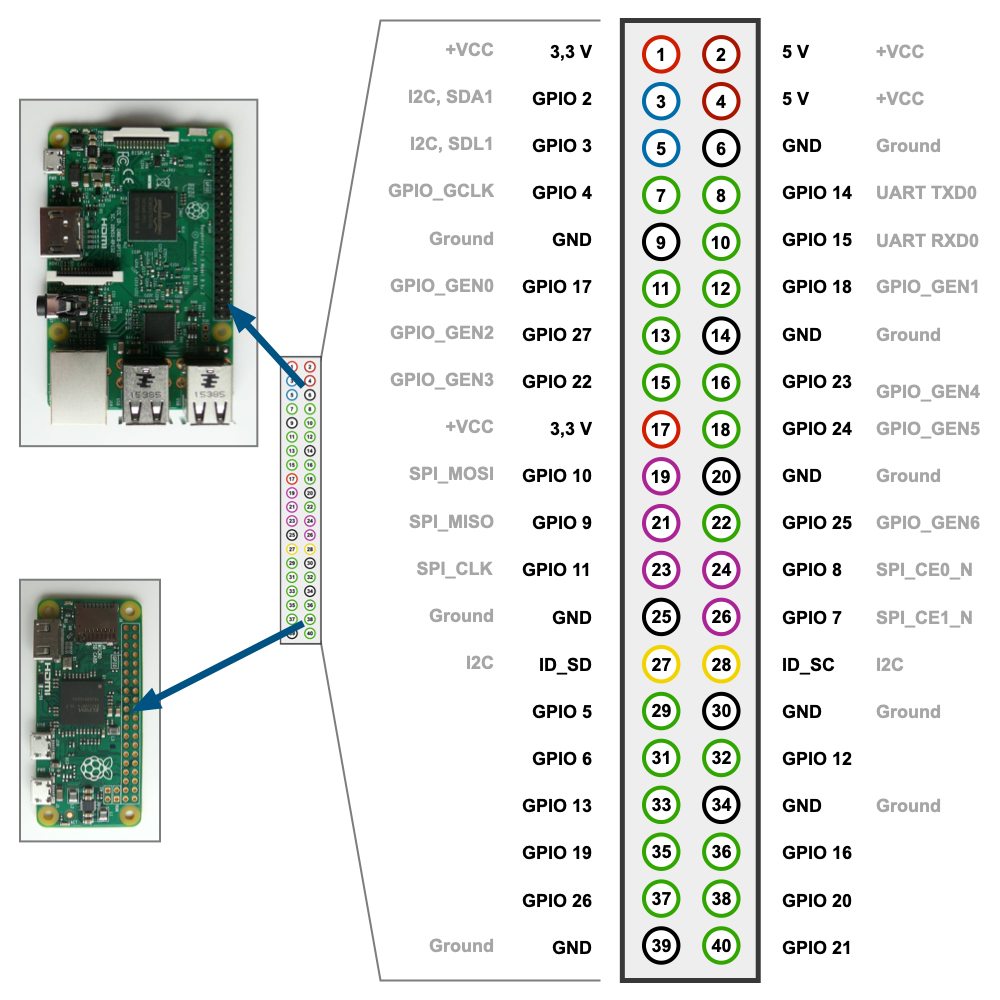
\includegraphics[width=10cm]{pics/GPIO.png}
  \caption{Belegung der GPIOs eines Raspberry Pi Model 4B / Raspberry Pi Zero}
  \cite{GPIOLayout}
\end{figure}
GPIOs sind empfindliche Schnittstellen, denn sie können schon bei geringen Stromstärken Schaden nehmen. Theoretisch ist eine Stromstärke von 16mA (Milliampere) möglich, wobei diese nie benötigt wird, da die GPIOs schon mit einer Stromstärke von 0.5mA geschalten werden können. Um die Langlebigkeit des Raspberry Pi zu gewährleisten, sollten nie mehr als 8mA von einem GPIO abgegeben werden. 
Es gibt jedoch Ausnahmen, wie die +5V-Pins. Diese bieten für externe Schaltungen eine Spannung bis zu 5V an, sind jedoch ebenfalls bei der Stromentnahme begrenzt. Hier wird mit etwa 25mA pro 5V-Pin gerechnet. Sollte dies für eine Schaltung nicht ausreichen, kann auf externe Stromquellen zurückgegriffen werden, wie eine Stromversorgung über ein separates Netzteil mit USB-Anschluss, oder die Versorgung über einen der verfügbaren USB-Ports des Raspberry Pi selbst. 

\cite{GPIO}
\subsubsection{NFC-Leser}
\subsubsection{Numpad [DH]}
Das Numpad ermöglicht der Benutzerin oder dem Benutzer die Eingabe eines 6-stelligen Zahlencodes. Dazu wird bei APERTA ein übliches Nummernfeld angeschlossen. Der eingegebe Code wird dann geprüft und mit den vorhandenen Codes in der Datenbank abgeglichen. Stimmen die Zahlenkombinationen überein, so öffnet sich das Garagentor. Zur Überprüfung wird der eingegebene Code auf dem LCD angezeigt. So kann sichergestellt werden, dass keine falschen Zahlen eingegeben werden. Sollte eine falsche Kombination vorliegen, dann wird auf dem Display eine Fehlermeldung ausgegeben.

\begin{figure}[h]
  \centering
  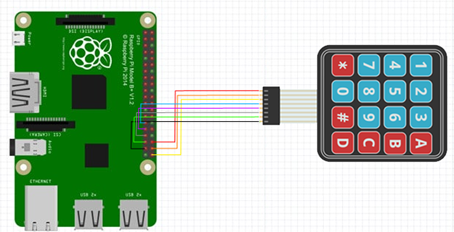
\includegraphics[width=0.8\textwidth]{pics/Nummerfeld.png}
  \caption{Abbildung eines Nummernfelds}
  \cite{Nummernfeld}
\end{figure}

\subsubsection{Kamera}
Die Kamera ermöglicht dem Raspberry Pi, die Kennzeichen zu sehen und darauf die Kennzeichen zu erkennen. Dazu wird bei APERTA eine handelsübliche Webcam verwendet, die über einen der beiden USB 3.0 Ports am Raspberry angeschlossen wird.
Um genug Auflösung für die Kennzeichenerkennung zu gewährleisten, wurde auf eine Webcam zurückgegriffen, welche mit bis zu 1920 Pixeln mal 1080 Pixeln aufnehmen kann.
Alternativ wäre auch eine Raspberry Pi Camera möglich gewesen, jedoch wurde die aufgrund ihres kurzen Flachbandkabels nicht verwendet, um die Kamera auch in größere Entfernung vom Raspberry Pi nutzen zu können.
\begin{figure}[H]
  \centering
  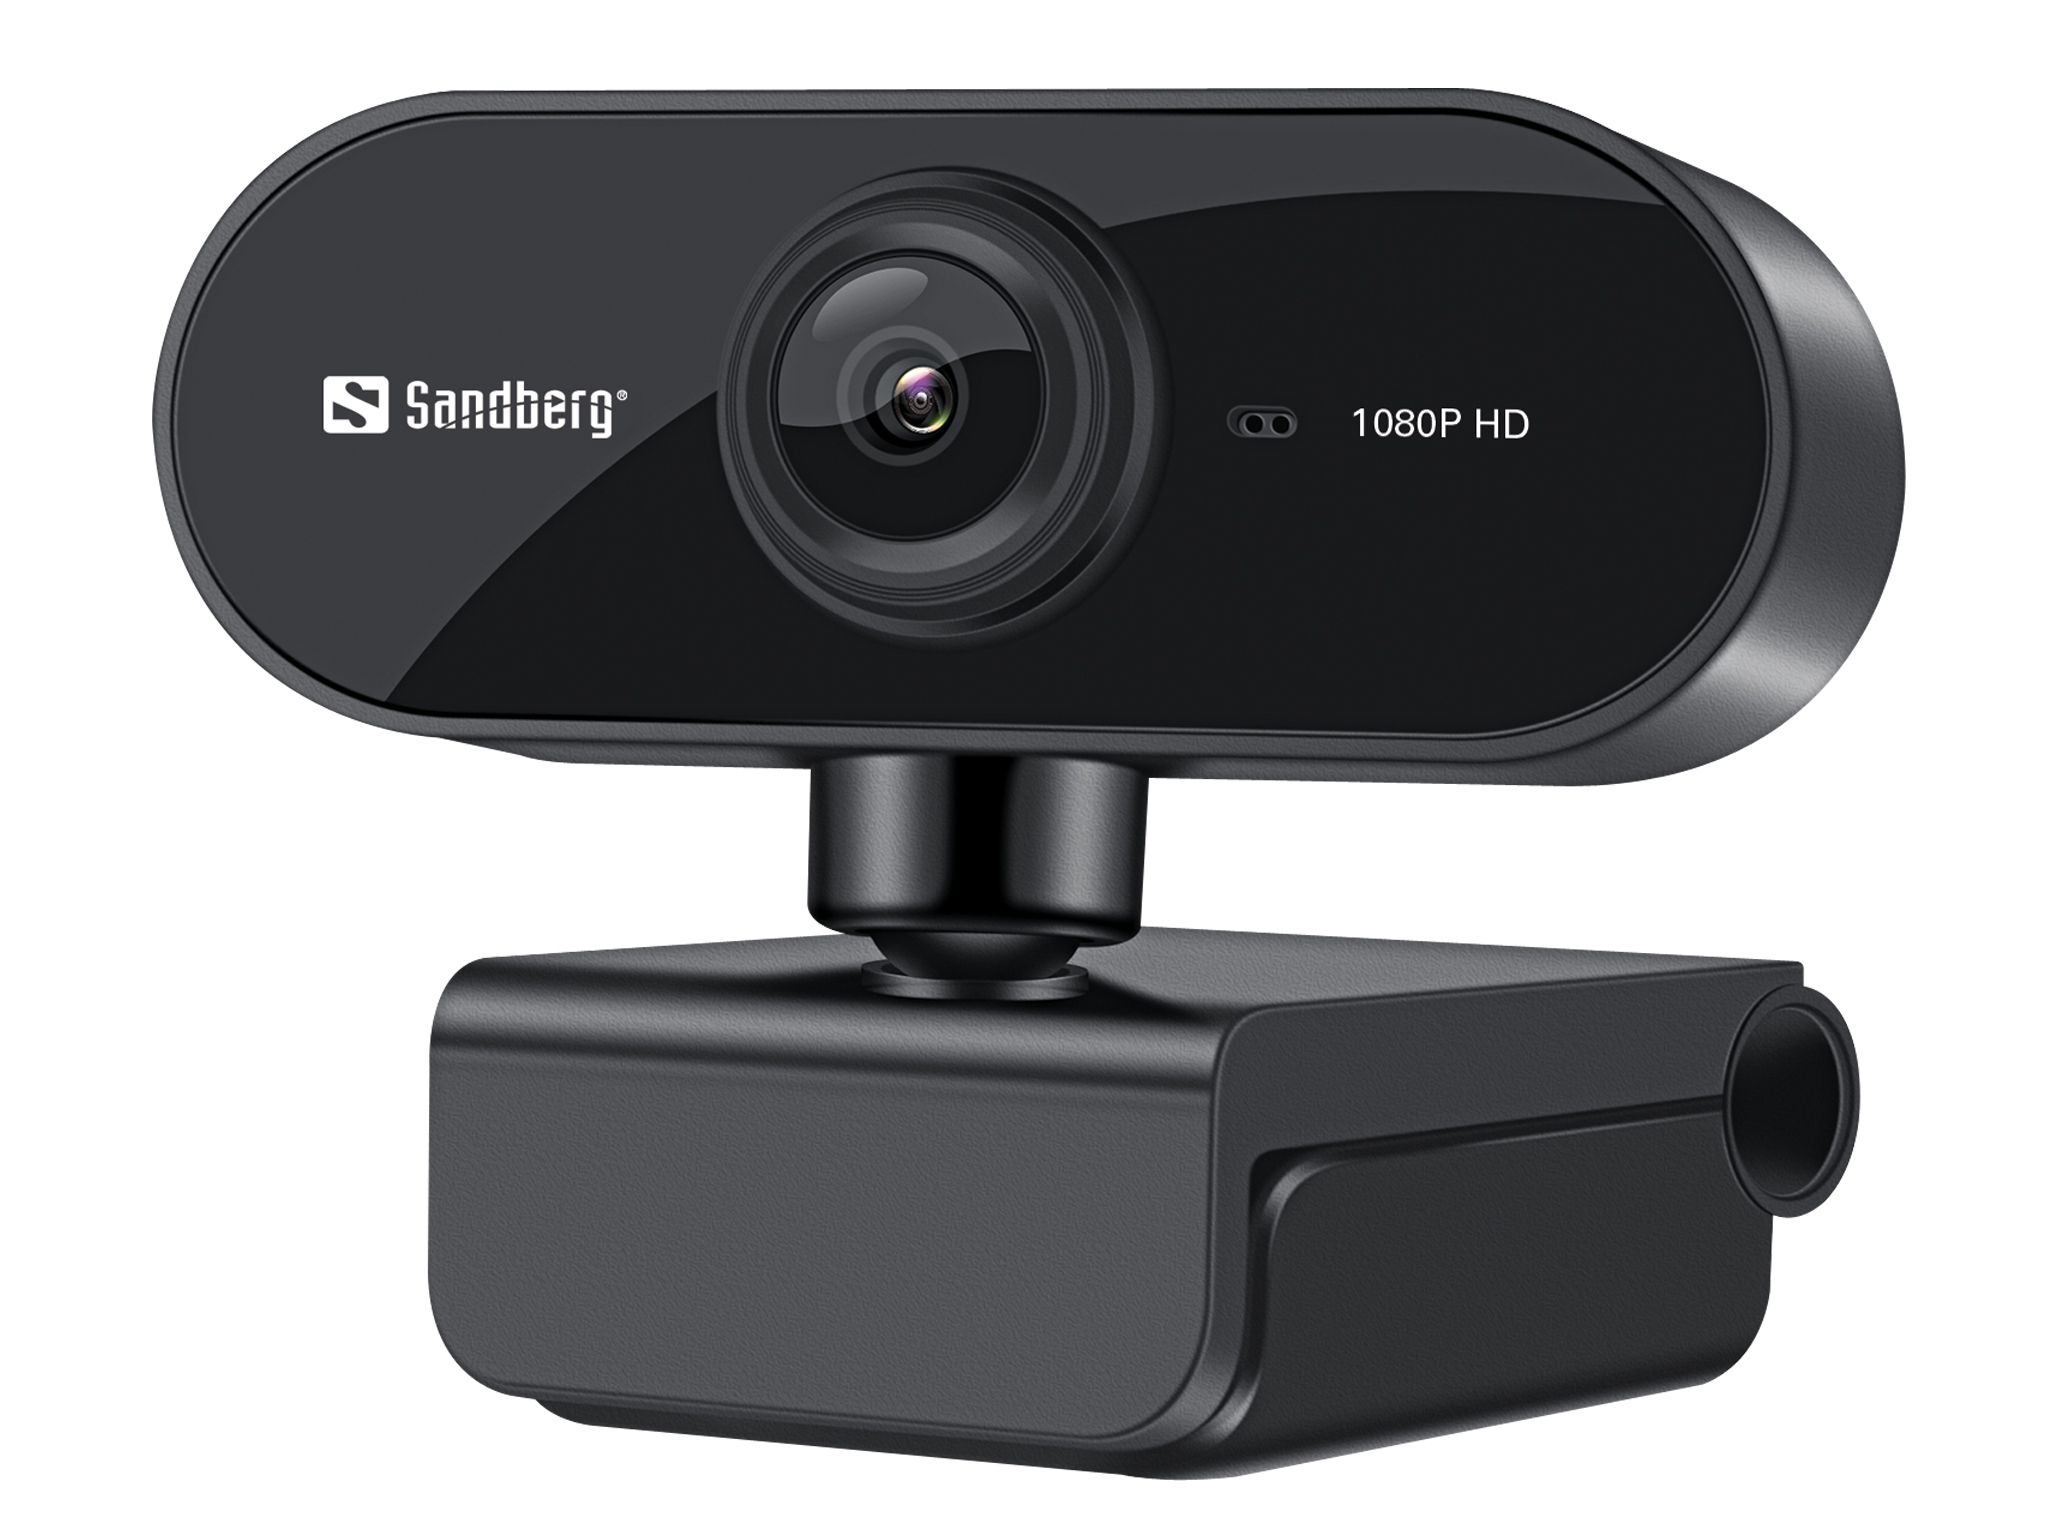
\includegraphics[width=8cm]{pics/Webcam.jpg}
  \caption{Webcam mit gleichen Spezifikationen}
  \cite{Webcam}
\end{figure}

\begin{figure}[H]
  \centering
  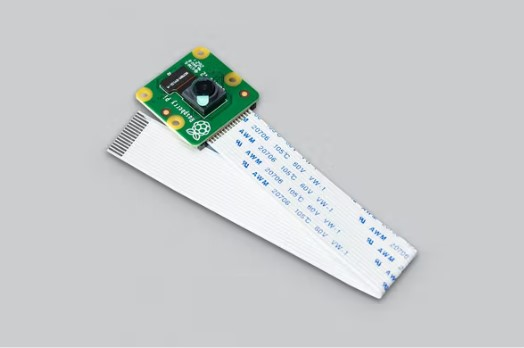
\includegraphics[width=8cm]{pics/RaspberryPiCameraModule2.jpg}
  \caption{Raspberry Pi Camera Module 2}
  \cite{PiCamera}
\end{figure}

\subsubsection{Display}
Um dem Nutzer oder der Nutzerin vor der Garage mitzuteilen, was gerade geschieht, wird ein Display verwendet, auf dem mitgeteilt wird, ob die Kombination, welche auf dem Nummernfeld eingegeben wurde korrekt ist, oder ob die NFC-Karte autorisiert ist.
Da auf diesem Display nur kurze Textausgaben angezeigt werden, fiel die Entscheidung auf ein LCD-Display, welches in zwei Zeilen beschrieben werden kann. Dieses bat zudem weitere Vorteile, wie die geringen Kosten von EUR 9,00 pro Stück, die Spannungsversorgung durch den Raspberry Pi selbst, sowie die einfache Möglichkeit, Text darauf auszugeben.
Im Lieferumfang des Displays war zudem ein I2C Serial Adapter, welcher durch seine 4 benötigten Ports um 8 Pins auf dem Raspberry Pi weniger braucht, als das direkt angeschlossene Display.
\cite{DifferentConnectionTypesDisplay}
\begin{figure}[H]
  \centering
  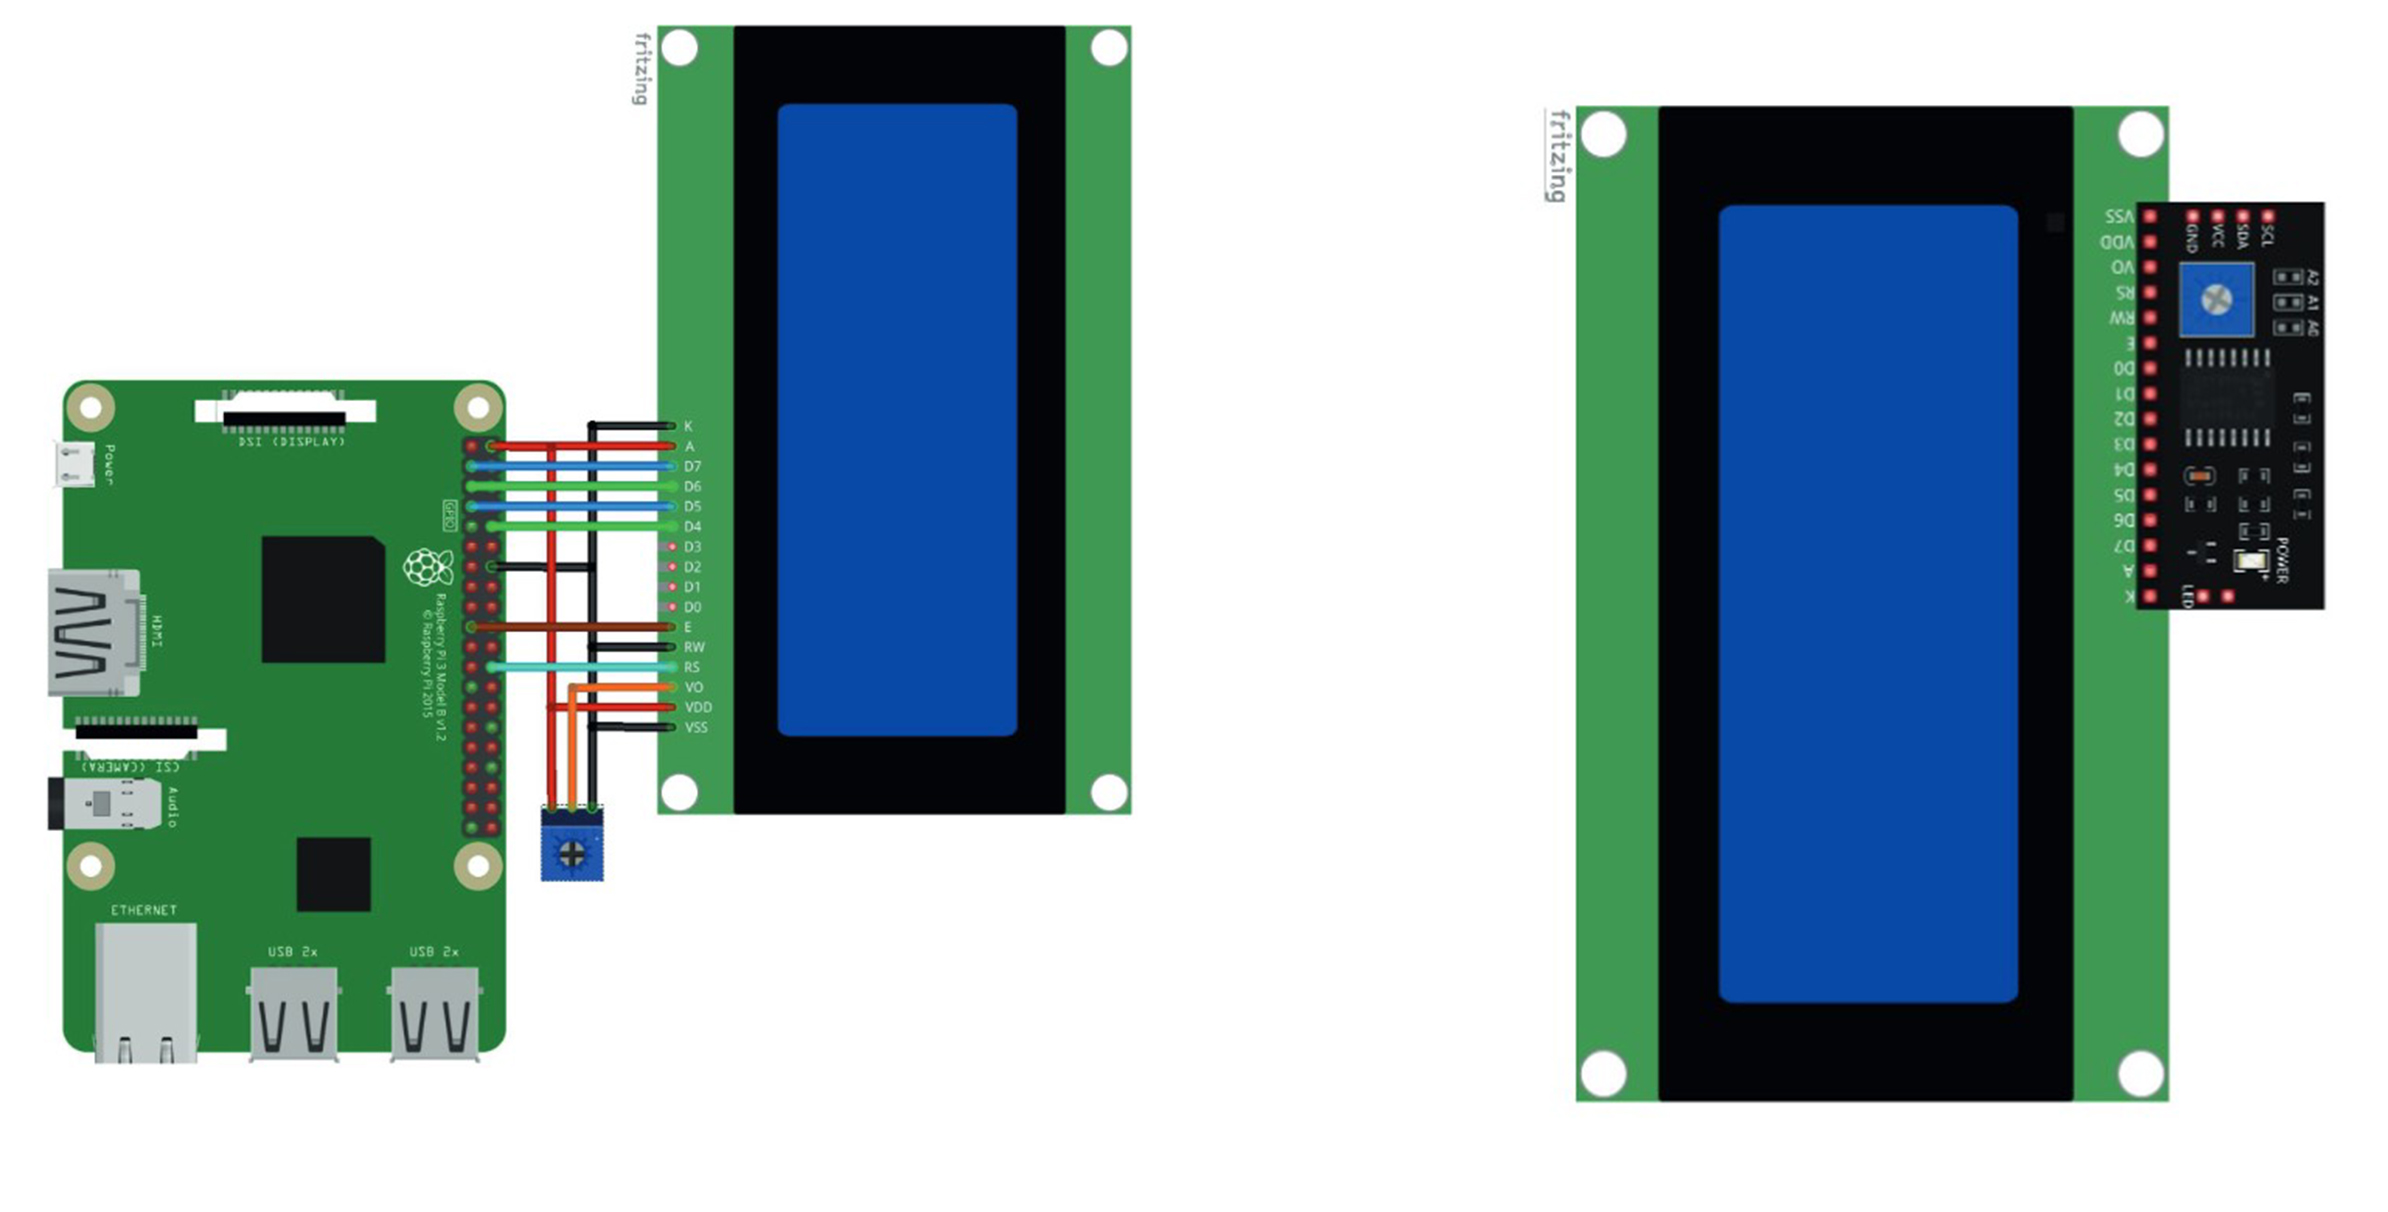
\includegraphics[width=15cm]{pics/DisplayComparison.jpg}
  \caption{Display direkt angeschlossen / Display über I2C Adapter angeschlossen}
\end{figure}
Die technischen Daten des Displays lauten:
\begin{itemize}
  \item 4 Zeilen zu je 20 Zeichen beschreibbar
  \item Blaue Hintergrundbeleuchtung
  \item 5V Versorgungsspannung
\end{itemize}
\cite{RaspberryDisplay}

 \subsubsection{Relais}
Handelsübliche Garagentore werden mit einer Spannung von 230 Volt betrieben. Der Raspberry Pi kann diese nicht direkt ansteuern, da die Spannung die interne Elektronik des Pi zerstören würde. Dennoch ist es nötig, wie bei einem Schalter den Steuerstromkreis des Garagentores zu schließen, um den Öffnungsmechanismus zu aktivieren. Um dies zu erreichen, wird ein Relais verwendet, welches in den externen Stromkreis geschalten wird und wie eine Brücke den Stromkreis schließen kann. Ein Relais besteht aus einer Spule aus Draht und einem Metallkern. Wird Strom durch den Draht geschickt, wird der Kern magnetisiert. Ohne Strom verschwindet das Magnetfeld des Kerns wieder.

Das Relais ist ein Elektromagnet, welcher durch den Steuerkreis einen Eisenanker zu sich zieht und somit den Arbeitsstromkreis schließt. Der Arbeitsstromkreis kann unabhängig vom Steuerkreis aufgebaut sein und auch unterschiedliche Spannungen und Stromstärken besitzen. Wichtig ist nur, dass das richtige Relais für den Arbeitskreis verwendet wird. Im Fall diese Projektes wird ein Relais verwendet, welches für bis zu 250 Volt Gleichstrom des Arbeitskreises verwendet werden kann.
\cite{Relais}
\begin{figure}[H]
  \centering
  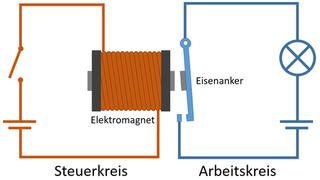
\includegraphics[width=8cm]{pics/Relais.png}
  \caption{Funktionsweise eines Relais als Schema}
  \cite{RelaisBild}
\end{figure}


\subsubsection{Steuerung der Hardware}
Um die Komponenten miteinander zu verbinden, war eine Programmiersprache notwendig, die mit den über GPIOs angeschlossenen Bauteilen kommunizieren kann. Dazu gab es eine Handvoll von Programmiersprachen, welche für die Entwicklung von Projekten mit dem Raspberry Pi in Frage kamen.

\begin{itemize}
  \item \textit{Scratch: }Scratch ist eine baukastenartige Programmiersprache, bei der Befehlsblöcke mithilfe der Maus aneinander angereiht werden. Entwickelt vom MIT Media Lab, richtet sich Scratch an Programmierneulinge und Kinder, welche es unterstützen soll, programmieren zu lernen, Code lesen und verstehen.
  \item \textit{Python: }Python zählt zu den meistverwendeten Programmiersprachen in Verbindung mit dem Raspberry Pi. Es zeichnet sich durch seine einsteigerfreundliche Syntax und die riesige Community aus, welche es ermöglicht, auf eine Vielzahl an Frameworks und Libraries zurückzugreifen. Python beschränkt sich dabei nicht auf einen bestimmten Einsatzbereich, sondern kann für die Entwicklung von graphischen Nutzeroberflächen, im Webdevelopment, zum Trainieren von Künstlichen Intelligenzen sowie für Automatisierung verwendet werden.
  \item \textit{JavaScript: } JavaScript ist nicht nur eine Erweiterung von HTML als Scripting Sprache, sondern viel mehr eine eigenständige, umfangreiche Programmiersprache. Sie wird meistens mit Webentwicklung in Verbindung gebracht, ist jedoch auch fähig, bereits bestehende Applikationen zu erweitern.
  \item \textit{Java: } Java ist eine der vielseitigsten Programmiersprachen, da sie erlaubt, unabhängig von Betriebssystem zu entwickeln, ohne den Code für jede Plattform verändern zu müssen. Mit mehr als 3 Milliarden Geräten, auf denen Java läuft, ist sie eine der meist verbreiteten Programmiersprachen.
  \item \textit{C: } C ist einer der stärksten Konkurrenten von Java. Raspbian OS, das Betriebssystem des Raspberry Pi, wurde beispielsweise in C geschrieben. C zeichnet sich durch einen klar strukturierten Programmierstil und die Möglichkeit, Arbeitsspeicher direkt anzusprechen, aus. Die Haupteinsatzgebiete von C sind die Entwicklung von Betriebssystemen und Compilern.
  \item \textit{C++: } Verglichen mit C, kann sich C++ mit objektorientierter Programmierung auszeichnen. Die Kombination aus prozeduraler und objektorientierterer Programmierung machen C++ zu einer Allzwecklösung, mit welcher von Betriebssystemen über Spiele bis hin zu Webbrowsern alles entwickelt werden kann.
  \item \textit{Perl: } Die Perl Org. hat mit Perl eine Sprache entwickelt, welche für fast jede Aufgabe, die mit C oder C++ Libraries zu tun hat, geeignet ist. Die große Auswahl an Libraries und Modulen sprechen trotz der geringen Bekanntheit für Perl, welche weiters für die Webentwicklung, Systemadministration, GUI-Entwicklung und vielem mehr verwendet werden kann.
  \item \textit{Erlang: } Erlang ist eine relativ unbekannte Sprache, da sie meist für Industrieapplikationen verwendet wird. Auszeichnungsmerkmale von Erlang sind beispielsweise die Fähigkeit, skalierbare Echtzeitsysteme zu entwickeln. Auch bei dezentralisierten Systemen ist Erlang eine gute Wahl, da das Programm bei Ausfall eines Rechners aus dem Cluster problemlos weiter arbeiten kann. Verwender sind unter anderem Banken und Telekommunikationsunternehmen.
\end{itemize}
\cite{RaspberryProgramming}\\
Durch die einfache Möglichkeit, mit den GPIOs zu arbeiten, sowie der einfach verständlichen Syntax, wurde Python verwendet. Das Team konnte somit zusätzlich auf bereits bestehende Kenntnisse aufbauen.

\subsubsection{RFID-Karte und -Leser [BG]}
\setauthor{Benjamin Golic}

Um den Zutritt zur Garage mittels RFID-Karte beziehungsweise RFID-Chip zu ermöglichen, wird ein RFID-Kit für den Raspberry Pi verwendet. Hierbei wird auf RFID-Kit der Firma AZ-Delivery gesetzt. Dieses Kit bietet den Vorteil, dass es eine eigene Library zur Programmierung der Funktionalität mit sich bringt. Für den geringen Preis von EUR 5,00 enthält das Kit einen RFID-Leser, eine RFID-Karte und einen RFID-Chip.
\cite{RFIDaz}\\

Eine Alternative zu dem RFID-Kit von AZ-Delivery wäre das Kit der Firma Makerfactory. Der höhere Preis und die geringere Anzahl an Komponenten sprachen gegen dieses Kit.
\cite{RFIDalternative}

\begin{figure}[H]
  \centering
  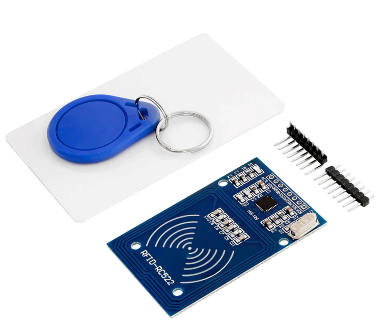
\includegraphics[width=0.4\textwidth]{pics/RFID-Kit-AZ.png}
  \caption{RFID-Kit der Firma AZ-Delivery}
  \cite{RFIDaz}
\end{figure}

\begin{figure}[H]
  \centering
  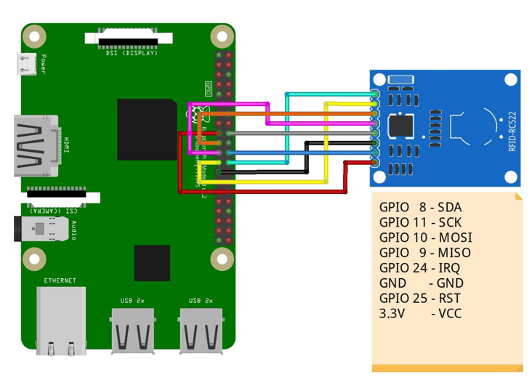
\includegraphics[width=0.4\textwidth]{pics/RFID-Schaltbild.png}
  \caption{Schaltbild des RFID-Lesers}
  \cite{RFIDschaltbild}
\end{figure}

